\documentclass[twoside]{article}
\usepackage{aistats2027}
\usepackage[round]{natbib}
\renewcommand{\bibname}{References}
\renewcommand{\bibsection}{\subsubsection*{\bibname}}
  
% Shared notation from the previous conference draft.
%%%%% NEW MATH DEFINITIONS %%%%%

\usepackage{amsmath,amsfonts,bm}

% Mark sections of captions for referring to divisions of figures
\newcommand{\figleft}{{\em (Left)}}
\newcommand{\figcenter}{{\em (Center)}}
\newcommand{\figright}{{\em (Right)}}
\newcommand{\figtop}{{\em (Top)}}
\newcommand{\figbottom}{{\em (Bottom)}}
\newcommand{\captiona}{{\em (a)}}
\newcommand{\captionb}{{\em (b)}}
\newcommand{\captionc}{{\em (c)}}
\newcommand{\captiond}{{\em (d)}}

% Highlight a newly defined term
\newcommand{\newterm}[1]{{\bf #1}}


% Figure reference, lower-case.
\def\figref#1{figure~\ref{#1}}
% Figure reference, capital. For start of sentence
\def\Figref#1{Figure~\ref{#1}}
\def\twofigref#1#2{figures \ref{#1} and \ref{#2}}
\def\quadfigref#1#2#3#4{figures \ref{#1}, \ref{#2}, \ref{#3} and \ref{#4}}
% Section reference, lower-case.
\def\secref#1{section~\ref{#1}}
% Section reference, capital.
\def\Secref#1{Section~\ref{#1}}
% Reference to two sections.
\def\twosecrefs#1#2{sections \ref{#1} and \ref{#2}}
% Reference to three sections.
\def\secrefs#1#2#3{sections \ref{#1}, \ref{#2} and \ref{#3}}
% Reference to an equation, lower-case.
\def\eqref#1{equation~\ref{#1}}
% Reference to an equation, upper case
\def\Eqref#1{Equation~\ref{#1}}
% A raw reference to an equation---avoid using if possible
\def\plaineqref#1{\ref{#1}}
% Reference to a chapter, lower-case.
\def\chapref#1{chapter~\ref{#1}}
% Reference to an equation, upper case.
\def\Chapref#1{Chapter~\ref{#1}}
% Reference to a range of chapters
\def\rangechapref#1#2{chapters\ref{#1}--\ref{#2}}
% Reference to an algorithm, lower-case.
\def\algref#1{algorithm~\ref{#1}}
% Reference to an algorithm, upper case.
\def\Algref#1{Algorithm~\ref{#1}}
\def\twoalgref#1#2{algorithms \ref{#1} and \ref{#2}}
\def\Twoalgref#1#2{Algorithms \ref{#1} and \ref{#2}}
% Reference to a part, lower case
\def\partref#1{part~\ref{#1}}
% Reference to a part, upper case
\def\Partref#1{Part~\ref{#1}}
\def\twopartref#1#2{parts \ref{#1} and \ref{#2}}

\def\ceil#1{\lceil #1 \rceil}
\def\floor#1{\lfloor #1 \rfloor}
\def\1{\bm{1}}
\newcommand{\train}{\mathcal{D}}
\newcommand{\valid}{\mathcal{D_{\mathrm{valid}}}}
\newcommand{\test}{\mathcal{D_{\mathrm{test}}}}

\def\eps{{\epsilon}}


% Random variables
\def\reta{{\textnormal{$\eta$}}}
\def\ra{{\textnormal{a}}}
\def\rb{{\textnormal{b}}}
\def\rc{{\textnormal{c}}}
\def\rd{{\textnormal{d}}}
\def\re{{\textnormal{e}}}
\def\rf{{\textnormal{f}}}
\def\rg{{\textnormal{g}}}
\def\rh{{\textnormal{h}}}
\def\ri{{\textnormal{i}}}
\def\rj{{\textnormal{j}}}
\def\rk{{\textnormal{k}}}
\def\rl{{\textnormal{l}}}
% rm is already a command, just don't name any random variables m
\def\rn{{\textnormal{n}}}
\def\ro{{\textnormal{o}}}
\def\rp{{\textnormal{p}}}
\def\rq{{\textnormal{q}}}
\def\rr{{\textnormal{r}}}
\def\rs{{\textnormal{s}}}
\def\rt{{\textnormal{t}}}
\def\ru{{\textnormal{u}}}
\def\rv{{\textnormal{v}}}
\def\rw{{\textnormal{w}}}
\def\rx{{\textnormal{x}}}
\def\ry{{\textnormal{y}}}
\def\rz{{\textnormal{z}}}

% Random vectors
\def\rvepsilon{{\mathbf{\epsilon}}}
\def\rvtheta{{\mathbf{\theta}}}
\def\rva{{\mathbf{a}}}
\def\rvb{{\mathbf{b}}}
\def\rvc{{\mathbf{c}}}
\def\rvd{{\mathbf{d}}}
\def\rve{{\mathbf{e}}}
\def\rvf{{\mathbf{f}}}
\def\rvg{{\mathbf{g}}}
\def\rvh{{\mathbf{h}}}
\def\rvu{{\mathbf{i}}}
\def\rvj{{\mathbf{j}}}
\def\rvk{{\mathbf{k}}}
\def\rvl{{\mathbf{l}}}
\def\rvm{{\mathbf{m}}}
\def\rvn{{\mathbf{n}}}
\def\rvo{{\mathbf{o}}}
\def\rvp{{\mathbf{p}}}
\def\rvq{{\mathbf{q}}}
\def\rvr{{\mathbf{r}}}
\def\rvs{{\mathbf{s}}}
\def\rvt{{\mathbf{t}}}
\def\rvu{{\mathbf{u}}}
\def\rvv{{\mathbf{v}}}
\def\rvw{{\mathbf{w}}}
\def\rvx{{\mathbf{x}}}
\def\rvy{{\mathbf{y}}}
\def\rvz{{\mathbf{z}}}

% Elements of random vectors
\def\erva{{\textnormal{a}}}
\def\ervb{{\textnormal{b}}}
\def\ervc{{\textnormal{c}}}
\def\ervd{{\textnormal{d}}}
\def\erve{{\textnormal{e}}}
\def\ervf{{\textnormal{f}}}
\def\ervg{{\textnormal{g}}}
\def\ervh{{\textnormal{h}}}
\def\ervi{{\textnormal{i}}}
\def\ervj{{\textnormal{j}}}
\def\ervk{{\textnormal{k}}}
\def\ervl{{\textnormal{l}}}
\def\ervm{{\textnormal{m}}}
\def\ervn{{\textnormal{n}}}
\def\ervo{{\textnormal{o}}}
\def\ervp{{\textnormal{p}}}
\def\ervq{{\textnormal{q}}}
\def\ervr{{\textnormal{r}}}
\def\ervs{{\textnormal{s}}}
\def\ervt{{\textnormal{t}}}
\def\ervu{{\textnormal{u}}}
\def\ervv{{\textnormal{v}}}
\def\ervw{{\textnormal{w}}}
\def\ervx{{\textnormal{x}}}
\def\ervy{{\textnormal{y}}}
\def\ervz{{\textnormal{z}}}

% Random matrices
\def\rmA{{\mathbf{A}}}
\def\rmB{{\mathbf{B}}}
\def\rmC{{\mathbf{C}}}
\def\rmD{{\mathbf{D}}}
\def\rmE{{\mathbf{E}}}
\def\rmF{{\mathbf{F}}}
\def\rmG{{\mathbf{G}}}
\def\rmH{{\mathbf{H}}}
\def\rmI{{\mathbf{I}}}
\def\rmJ{{\mathbf{J}}}
\def\rmK{{\mathbf{K}}}
\def\rmL{{\mathbf{L}}}
\def\rmM{{\mathbf{M}}}
\def\rmN{{\mathbf{N}}}
\def\rmO{{\mathbf{O}}}
\def\rmP{{\mathbf{P}}}
\def\rmQ{{\mathbf{Q}}}
\def\rmR{{\mathbf{R}}}
\def\rmS{{\mathbf{S}}}
\def\rmT{{\mathbf{T}}}
\def\rmU{{\mathbf{U}}}
\def\rmV{{\mathbf{V}}}
\def\rmW{{\mathbf{W}}}
\def\rmX{{\mathbf{X}}}
\def\rmY{{\mathbf{Y}}}
\def\rmZ{{\mathbf{Z}}}

% Elements of random matrices
\def\ermA{{\textnormal{A}}}
\def\ermB{{\textnormal{B}}}
\def\ermC{{\textnormal{C}}}
\def\ermD{{\textnormal{D}}}
\def\ermE{{\textnormal{E}}}
\def\ermF{{\textnormal{F}}}
\def\ermG{{\textnormal{G}}}
\def\ermH{{\textnormal{H}}}
\def\ermI{{\textnormal{I}}}
\def\ermJ{{\textnormal{J}}}
\def\ermK{{\textnormal{K}}}
\def\ermL{{\textnormal{L}}}
\def\ermM{{\textnormal{M}}}
\def\ermN{{\textnormal{N}}}
\def\ermO{{\textnormal{O}}}
\def\ermP{{\textnormal{P}}}
\def\ermQ{{\textnormal{Q}}}
\def\ermR{{\textnormal{R}}}
\def\ermS{{\textnormal{S}}}
\def\ermT{{\textnormal{T}}}
\def\ermU{{\textnormal{U}}}
\def\ermV{{\textnormal{V}}}
\def\ermW{{\textnormal{W}}}
\def\ermX{{\textnormal{X}}}
\def\ermY{{\textnormal{Y}}}
\def\ermZ{{\textnormal{Z}}}

% Vectors
\def\vzero{{\bm{0}}}
\def\vone{{\bm{1}}}
\def\vmu{{\bm{\mu}}}
\def\vtheta{{\bm{\theta}}}
\def\va{{\bm{a}}}
\def\vb{{\bm{b}}}
\def\vc{{\bm{c}}}
\def\vd{{\bm{d}}}
\def\ve{{\bm{e}}}
\def\vf{{\bm{f}}}
\def\vg{{\bm{g}}}
\def\vh{{\bm{h}}}
\def\vi{{\bm{i}}}
\def\vj{{\bm{j}}}
\def\vk{{\bm{k}}}
\def\vl{{\bm{l}}}
\def\vm{{\bm{m}}}
\def\vn{{\bm{n}}}
\def\vo{{\bm{o}}}
\def\vp{{\bm{p}}}
\def\vq{{\bm{q}}}
\def\vr{{\bm{r}}}
\def\vs{{\bm{s}}}
\def\vt{{\bm{t}}}
\def\vu{{\bm{u}}}
\def\vv{{\bm{v}}}
\def\vw{{\bm{w}}}
\def\vx{{\bm{x}}}
\def\vy{{\bm{y}}}
\def\vz{{\bm{z}}}

% Elements of vectors
\def\evalpha{{\alpha}}
\def\evbeta{{\beta}}
\def\evepsilon{{\epsilon}}
\def\evlambda{{\lambda}}
\def\evomega{{\omega}}
\def\evmu{{\mu}}
\def\evpsi{{\psi}}
\def\evsigma{{\sigma}}
\def\evtheta{{\theta}}
\def\eva{{a}}
\def\evb{{b}}
\def\evc{{c}}
\def\evd{{d}}
\def\eve{{e}}
\def\evf{{f}}
\def\evg{{g}}
\def\evh{{h}}
\def\evi{{i}}
\def\evj{{j}}
\def\evk{{k}}
\def\evl{{l}}
\def\evm{{m}}
\def\evn{{n}}
\def\evo{{o}}
\def\evp{{p}}
\def\evq{{q}}
\def\evr{{r}}
\def\evs{{s}}
\def\evt{{t}}
\def\evu{{u}}
\def\evv{{v}}
\def\evw{{w}}
\def\evx{{x}}
\def\evy{{y}}
\def\evz{{z}}

% Matrix
\def\mA{{\bm{A}}}
\def\mB{{\bm{B}}}
\def\mC{{\bm{C}}}
\def\mD{{\bm{D}}}
\def\mE{{\bm{E}}}
\def\mF{{\bm{F}}}
\def\mG{{\bm{G}}}
\def\mH{{\bm{H}}}
\def\mI{{\bm{I}}}
\def\mJ{{\bm{J}}}
\def\mK{{\bm{K}}}
\def\mL{{\bm{L}}}
\def\mM{{\bm{M}}}
\def\mN{{\bm{N}}}
\def\mO{{\bm{O}}}
\def\mP{{\bm{P}}}
\def\mQ{{\bm{Q}}}
\def\mR{{\bm{R}}}
\def\mS{{\bm{S}}}
\def\mT{{\bm{T}}}
\def\mU{{\bm{U}}}
\def\mV{{\bm{V}}}
\def\mW{{\bm{W}}}
\def\mX{{\bm{X}}}
\def\mY{{\bm{Y}}}
\def\mZ{{\bm{Z}}}
\def\mBeta{{\bm{\beta}}}
\def\mPhi{{\bm{\Phi}}}
\def\mLambda{{\bm{\Lambda}}}
\def\mSigma{{\bm{\Sigma}}}

% Tensor
\DeclareMathAlphabet{\mathsfit}{\encodingdefault}{\sfdefault}{m}{sl}
\SetMathAlphabet{\mathsfit}{bold}{\encodingdefault}{\sfdefault}{bx}{n}
\newcommand{\tens}[1]{\bm{\mathsfit{#1}}}
\def\tA{{\tens{A}}}
\def\tB{{\tens{B}}}
\def\tC{{\tens{C}}}
\def\tD{{\tens{D}}}
\def\tE{{\tens{E}}}
\def\tF{{\tens{F}}}
\def\tG{{\tens{G}}}
\def\tH{{\tens{H}}}
\def\tI{{\tens{I}}}
\def\tJ{{\tens{J}}}
\def\tK{{\tens{K}}}
\def\tL{{\tens{L}}}
\def\tM{{\tens{M}}}
\def\tN{{\tens{N}}}
\def\tO{{\tens{O}}}
\def\tP{{\tens{P}}}
\def\tQ{{\tens{Q}}}
\def\tR{{\tens{R}}}
\def\tS{{\tens{S}}}
\def\tT{{\tens{T}}}
\def\tU{{\tens{U}}}
\def\tV{{\tens{V}}}
\def\tW{{\tens{W}}}
\def\tX{{\tens{X}}}
\def\tY{{\tens{Y}}}
\def\tZ{{\tens{Z}}}


% Graph
\def\gA{{\mathcal{A}}}
\def\gB{{\mathcal{B}}}
\def\gC{{\mathcal{C}}}
\def\gD{{\mathcal{D}}}
\def\gE{{\mathcal{E}}}
\def\gF{{\mathcal{F}}}
\def\gG{{\mathcal{G}}}
\def\gH{{\mathcal{H}}}
\def\gI{{\mathcal{I}}}
\def\gJ{{\mathcal{J}}}
\def\gK{{\mathcal{K}}}
\def\gL{{\mathcal{L}}}
\def\gM{{\mathcal{M}}}
\def\gN{{\mathcal{N}}}
\def\gO{{\mathcal{O}}}
\def\gP{{\mathcal{P}}}
\def\gQ{{\mathcal{Q}}}
\def\gR{{\mathcal{R}}}
\def\gS{{\mathcal{S}}}
\def\gT{{\mathcal{T}}}
\def\gU{{\mathcal{U}}}
\def\gV{{\mathcal{V}}}
\def\gW{{\mathcal{W}}}
\def\gX{{\mathcal{X}}}
\def\gY{{\mathcal{Y}}}
\def\gZ{{\mathcal{Z}}}

% Sets
\def\sA{{\mathbb{A}}}
\def\sB{{\mathbb{B}}}
\def\sC{{\mathbb{C}}}
\def\sD{{\mathbb{D}}}
% Don't use a set called E, because this would be the same as our symbol
% for expectation.
\def\sF{{\mathbb{F}}}
\def\sG{{\mathbb{G}}}
\def\sH{{\mathbb{H}}}
\def\sI{{\mathbb{I}}}
\def\sJ{{\mathbb{J}}}
\def\sK{{\mathbb{K}}}
\def\sL{{\mathbb{L}}}
\def\sM{{\mathbb{M}}}
\def\sN{{\mathbb{N}}}
\def\sO{{\mathbb{O}}}
\def\sP{{\mathbb{P}}}
\def\sQ{{\mathbb{Q}}}
\def\sR{{\mathbb{R}}}
\def\sS{{\mathbb{S}}}
\def\sT{{\mathbb{T}}}
\def\sU{{\mathbb{U}}}
\def\sV{{\mathbb{V}}}
\def\sW{{\mathbb{W}}}
\def\sX{{\mathbb{X}}}
\def\sY{{\mathbb{Y}}}
\def\sZ{{\mathbb{Z}}}

% Entries of a matrix
\def\emLambda{{\Lambda}}
\def\emA{{A}}
\def\emB{{B}}
\def\emC{{C}}
\def\emD{{D}}
\def\emE{{E}}
\def\emF{{F}}
\def\emG{{G}}
\def\emH{{H}}
\def\emI{{I}}
\def\emJ{{J}}
\def\emK{{K}}
\def\emL{{L}}
\def\emM{{M}}
\def\emN{{N}}
\def\emO{{O}}
\def\emP{{P}}
\def\emQ{{Q}}
\def\emR{{R}}
\def\emS{{S}}
\def\emT{{T}}
\def\emU{{U}}
\def\emV{{V}}
\def\emW{{W}}
\def\emX{{X}}
\def\emY{{Y}}
\def\emZ{{Z}}
\def\emSigma{{\Sigma}}

% entries of a tensor
% Same font as tensor, without \bm wrapper
\newcommand{\etens}[1]{\mathsfit{#1}}
\def\etLambda{{\etens{\Lambda}}}
\def\etA{{\etens{A}}}
\def\etB{{\etens{B}}}
\def\etC{{\etens{C}}}
\def\etD{{\etens{D}}}
\def\etE{{\etens{E}}}
\def\etF{{\etens{F}}}
\def\etG{{\etens{G}}}
\def\etH{{\etens{H}}}
\def\etI{{\etens{I}}}
\def\etJ{{\etens{J}}}
\def\etK{{\etens{K}}}
\def\etL{{\etens{L}}}
\def\etM{{\etens{M}}}
\def\etN{{\etens{N}}}
\def\etO{{\etens{O}}}
\def\etP{{\etens{P}}}
\def\etQ{{\etens{Q}}}
\def\etR{{\etens{R}}}
\def\etS{{\etens{S}}}
\def\etT{{\etens{T}}}
\def\etU{{\etens{U}}}
\def\etV{{\etens{V}}}
\def\etW{{\etens{W}}}
\def\etX{{\etens{X}}}
\def\etY{{\etens{Y}}}
\def\etZ{{\etens{Z}}}

% The true underlying data generating distribution
\newcommand{\pdata}{p_{\rm{data}}}
% The empirical distribution defined by the training set
\newcommand{\ptrain}{\hat{p}_{\rm{data}}}
\newcommand{\Ptrain}{\hat{P}_{\rm{data}}}
% The model distribution
\newcommand{\pmodel}{p_{\rm{model}}}
\newcommand{\Pmodel}{P_{\rm{model}}}
\newcommand{\ptildemodel}{\tilde{p}_{\rm{model}}}
% Stochastic autoencoder distributions
\newcommand{\pencode}{p_{\rm{encoder}}}
\newcommand{\pdecode}{p_{\rm{decoder}}}
\newcommand{\precons}{p_{\rm{reconstruct}}}

\newcommand{\laplace}{\mathrm{Laplace}} % Laplace distribution

\newcommand{\E}{\mathbb{E}}
\newcommand{\Ls}{\mathcal{L}}
\newcommand{\R}{\mathbb{R}}
\newcommand{\emp}{\tilde{p}}
\newcommand{\lr}{\alpha}
\newcommand{\reg}{\lambda}
\newcommand{\rect}{\mathrm{rectifier}}
\newcommand{\softmax}{\mathrm{softmax}}
\newcommand{\sigmoid}{\sigma}
\newcommand{\softplus}{\zeta}
\newcommand{\KL}{D_{\mathrm{KL}}}
\newcommand{\Var}{\mathrm{Var}}
\newcommand{\standarderror}{\mathrm{SE}}
\newcommand{\Cov}{\mathrm{Cov}}
% Wolfram Mathworld says $L^2$ is for function spaces and $\ell^2$ is for vectors
% But then they seem to use $L^2$ for vectors throughout the site, and so does
% wikipedia.
\newcommand{\normlzero}{L^0}
\newcommand{\normlone}{L^1}
\newcommand{\normltwo}{L^2}
\newcommand{\normlp}{L^p}
\newcommand{\normmax}{L^\infty}

\newcommand{\parents}{Pa} % See usage in notation.tex. Chosen to match Daphne's book.

\DeclareMathOperator*{\argmax}{arg\,max}
\DeclareMathOperator*{\argmin}{arg\,min}

\DeclareMathOperator{\sign}{sign}
\DeclareMathOperator{\Tr}{Tr}
\let\ab\allowbreak


\usepackage{amsmath,amssymb,amsthm,mathtools}
\usepackage{booktabs}
\usepackage{tabularx}
\usepackage{graphicx}
\usepackage{capt-of}
\usepackage{placeins}
\usepackage{float}
\usepackage{needspace}
\usepackage{microtype}
\usepackage{xspace}
\usepackage{hyperref}
\usepackage{url}
\hypersetup{hidelinks}

\newcommand{\method}{KronHiPPO-STGP\xspace}
\newcommand{\trans}{\mathsf T}
\newtheorem{proposition}{Proposition}
\newtheorem{lemma}{Lemma}
\newtheorem{theorem}{Theorem}
\newtheorem{corollary}{Corollary}

\begin{document}

\twocolumn[
\aistatstitle{KronHiPPO-STGP: Online Bayesian Spatio-temporal Modelling with Evolving Memory}
\aistatsauthor{Anonymous Authors}
\aistatsaddress{Anonymous Institution}
]

\begin{abstract}\small\setlength{\emergencystretch}{1em}
Online Bayesian inference requires updating posterior beliefs while storing only a bounded summary of historical observations. Existing streaming approaches compress past data into finite states, but these states are usually constructed under a fixed representation. When latent parameters are updated or inducing coordinates change, the stored state may no longer correspond to the original likelihood contribution. We study this issue in online spatio-temporal Gaussian processes with evolving finite-dimensional representations. We propose \method, a method that maintains a bounded Gaussian likelihood state for a parametric mean component and a residual Gaussian process. The proposed state supports posterior updates after representation changes by transferring likelihood factors between successive HiPPO inducing coordinates without replaying previous observations. We derive three properties of evolving Bayesian memory: the cross information required to update coupled trend and residual components, the finite-dimensional projection operator between changing representations together with its associated information loss, and the conditions under which likelihood transfer preserves Kronecker structure. Based on these results, we develop a Schur--Sylvester posterior recovery procedure that is equivalent to solving the corresponding projected Gaussian system while avoiding dense matrix operations. Experiments on environmental, public-health, and traffic datasets show that \method maintains memory cost independent of stream length and achieves accurate prediction with calibrated uncertainty under online representation changes.
\end{abstract}

\section{Introduction}

Online Bayesian models must update predictions as new observations arrive while discarding raw historical data. This requirement imposes a memory constraint: the retained state must preserve uncertainty about past observations while remaining fixed in size as the stream grows.

Many real-world systems, including environmental monitoring, public health surveillance, and urban sensing, generate continuously arriving spatio-temporal observations where uncertainty quantification is required \citep{Hamelijnck2021,Silk2023,Li2018DCRNN}. Gaussian processes (GPs) provide a natural framework for this setting because they represent uncertainty over latent functions and capture dependencies across space and time \citep{Rasmussen2006,Hartikainen2011,Hamelijnck2021}. However, exact GP inference requires computation and storage that increase with the number of observations. Online GP methods therefore replace raw observations with finite representations, such as inducing variables or approximate likelihood factors \citep{Titsias2009,Matthews2016,Csato2002,Bui2017,Maddox2021}.

Streaming GP methods and sparse variational approaches maintain finite summaries of historical observations. These methods assume that the representation used to store the summary remains consistent during future updates. When the representation changes, however, the stored statistics may no longer describe the same latent quantities.

This issue arises naturally in online models with adaptive finite representations. The posterior update itself remains standard, but the Bayesian information accumulated in previous representations must be mapped to the current representation before further inference.

A decomposition into a parametric trend component and a correlated Gaussian process residual is a standard formulation in spatial statistics and Gaussian process modelling, including universal kriging and Bayesian spatial models \citep{Cressie1993,Stein1999,Rasmussen2006}. In this formulation,
\[
y=\phi^\top\beta+f .
\]
the trend component captures systematic variations explained by covariates, while the residual GP models remaining structured spatio-temporal dependencies \citep{Hamelijnck2021}.

While this decomposition is well established for offline inference, replay-free online learning introduces a different memory problem. Historical residual statistics depend on the trend parameters used during compression, so updating the mean component changes the interpretation of previously stored residual evidence. A bounded online state must therefore preserve trend--residual coupling information to support posterior revision after historical observations are discarded.

Maintaining long-range temporal information with a fixed number of variables has recently been studied through structured temporal representations such as HiPPO. HiPPO compresses the history of a signal into a fixed-dimensional state and has been used in long-range sequence models including S4 and Mamba \citep{Gu2020,Gu2022S4,GuDao2023Mamba}.

Recurrent Memory for Online Interdomain Gaussian Processes introduced HiPPO as a temporal interdomain inducing representation for Gaussian processes and showed that HiPPO-based inducing variables can preserve long-range temporal information with a fixed number of variables \citep{Chen2025}. Following this direction, we use HiPPO inducing representations for spatio-temporal Gaussian processes to maintain a compact temporal representation during online inference.

Unlike conventional inducing variables with fixed basis functions, HiPPO inducing variables depend on horizon-specific projection functions. As the temporal horizon expands, the inducing basis changes, and previously stored likelihood statistics must be interpreted in the updated representation \citep{Gu2020,Chen2025}.

Therefore, fixed dimensionality does not guarantee that two inducing states represent the same GP functionals. This representation change creates a Bayesian memory problem: historical likelihood information must be transferred before posterior inference continues.

The changing representation introduces three requirements for online Bayesian inference. First, updating the parametric mean requires retaining the coupling between trend and residual components. A residual-only summary cannot correct historical evidence after mean revision. Second, historical likelihood information must be transferred between successive inducing representations rather than reused directly. Third, the transferred likelihood must preserve exploitable structure to allow efficient recovery of the posterior over spatio-temporal inducing variables.

We introduce \method, a bounded-state Bayesian inference framework for online Gaussian processes with changing finite representations. The maintained state is a joint Gaussian likelihood factor over the parametric mean and residual inducing variables. It stores: (1) trend--residual coupling information for updating historical evidence after mean revisions; (2) likelihood statistics that can be transferred between successive HiPPO inducing representations; and (3) structured residual factors for efficient posterior recovery.

Our contributions are:
\begin{itemize}

\item We formulate online GP inference with changing inducing
representations by maintaining a joint Gaussian likelihood state over
trend and residual components.

\item We derive likelihood transfer between successive HiPPO
representations and characterize the associated projection loss. Under
the stated assumptions, the transferred likelihood preserves
Kronecker structure and admits efficient posterior recovery.

\item We evaluate the proposed framework on three real-world
spatio-temporal datasets and analyze the effects of memory revision,
representation transfer, and structured recovery.

\end{itemize}

\section{Related work}

\textbf{Finite Bayesian memory for online GP inference.}
Online GP inference replaces the growing observation history with finite
representations of past information. Sparse variational GPs achieve this
through inducing variables while preserving the GP conditional structure
\citep{Titsias2009,Matthews2016}. Interdomain inducing variables extend
this framework by representing latent functions through general linear
functionals rather than point evaluations
\citep{LazaroGredilla2009,VanderWilk2020}.

Streaming GP methods maintain sequential updates by storing posterior or
approximate likelihood summaries instead of raw observations
\citep{Csato2002,Bui2017,Maddox2021}. These methods focus on constructing
compact representations of historical information. In contrast, our
setting considers online inference where the inducing representation
itself changes, requiring the stored likelihood statistics to be
transferred before further updates.


\textbf{HiPPO representations and evolving inducing variables.}
HiPPO constructs fixed-dimensional states by projecting sequential
signals onto polynomial bases, providing a mechanism for long-range
memory compression \citep{Gu2020}. This idea has been adopted in deep
sequence models including S4 and Mamba
\citep{Gu2022S4,GuDao2023Mamba}. 

Recent work on recurrent memory for online interdomain Gaussian
processes introduces HiPPO projections as temporal inducing variables
and demonstrates their ability to retain long-range temporal
information with a fixed number of variables
\citep{Chen2025}. We adopt this type of temporal interdomain
representation for spatio-temporal GP inference. Unlike conventional
inducing variables with fixed basis functions, HiPPO inducing variables
depend on the temporal horizon. Therefore, online updates require
transforming historical likelihood information between successive
inducing representations.


\textbf{Structured inference for spatio-temporal GP.}
Scalable spatio-temporal GP inference commonly exploits structural
properties of covariance functions or latent representations.
State-space formulations use temporal Markov structure for efficient
inference \citep{Hartikainen2010,Nickisch2018}, while variational
approaches combine temporal structure with sparse spatial
representations \citep{Adam2020,Hamelijnck2021}. Kronecker methods
exploit spatial--temporal separability to reduce computation on product
grids \citep{VanLoan2000,Flaxman2015}.

Our work differs from these approaches by studying whether the
Kronecker structure is preserved after transporting a Bayesian
likelihood state between changing temporal inducing representations,
rather than assuming a fixed representation throughout inference.

\section{Preliminaries}

We first define the online information boundary, the joint trend--residual state, and the finite representation that evolves during inference.

\subsection{Online inference with bounded information}

We consider a sequential Bayesian inference problem in which data arrive in blocks. At block $k$, observations are available only at a subset of locations $V_k$, and predictions are required at held-out locations $Q_k$ before their values are revealed.

The online constraint is strict: after processing block $k$, raw observations from previous blocks are discarded. The inference procedure must therefore maintain a bounded state $\mathcal S_k$ that contains all information required for future posterior updates. Dataset-specific calibration and evaluation details are given in Section~5 and Appendix~B.

The representation defining $\mathcal S_k$ is allowed to change across updates, which distinguishes this setting from fixed-coordinate streaming inference.

\subsection{Trend--residual Bayesian state}

We model observations using a parametric component for known covariate effects and a residual Gaussian process:
\begin{equation}
 y(t,s)=\phi(t,s)^{\trans}\beta+f(t,s)+\epsilon,
 \qquad \epsilon\sim\mathcal N(0,\sigma_y^2).
 \label{eq:intro-model}
\end{equation}
The coefficient $\beta$ is a static latent variable,
$\beta\sim\mathcal N(m_{\beta,0},S_{\beta,0})$. Online learning updates its posterior but does not posit coefficient drift. The residual process $f$ captures correlated spatio-temporal variation through the separable kernel
\begin{equation}
 k((t,s),(t',s'))=k_t(t,t')k_s(s,s').
 \label{eq:separable}
\end{equation}
\subsection{Evolving finite representations}

To obtain bounded memory, we represent the residual process using finite interdomain variables. For temporal horizon $\mathcal H_k=[t_0,t_k]$, HiPPO defines inducing variables. For spatial inducing locations $z_j$, the mixed interdomain variables are
\begin{multline}
 u_{m,j}^{(k)}=\int_{\mathcal H_k} f(t,z_j)\psi_m(t;\mathcal H_k)\,dt,
 \\
 m=0,\ldots,M_t-1,\qquad j=1,\ldots,M_s.
 \label{eq:hippo-functional}
\end{multline}
The number of stored coefficients remains fixed as the horizon grows. However, the representation itself changes because the projection functions $\psi_m(t;\mathcal H_k)$ depend on the current horizon. Consequently,

\[
\dim(u_{k-1})=\dim(u_k)
\]

does not imply $u_{k-1}=u_k$. The two vectors have the same dimension but represent different GP functionals. The inducing-variable prior and conditional-mean projection matrix are
\begin{equation}
 p(u_k)=\mathcal N(0,K_{t,k}\otimes K_s),
 \qquad A_k=P_{t,k}\otimes C.
 \label{eq:inducing}
\end{equation}
Here $A_k$ maps the interdomain inducing variables to the conditional mean of the latent function values at the observation locations. These inducing variables parameterise the finite-dimensional variational approximation, while the full GP conditional is retained:
\begin{align}
 p(f_k\mid u_k)&=\mathcal N(A_ku_k,K_{f_kf_k}-Q_{f_kf_k}),\\
 q_k(\beta,u_k,f_k)&=p(f_k\mid u_k)q_k(\beta,u_k).
 \label{eq:vfe-family}
\end{align}
For fixed $(\beta,u_k)$, taking expectation over the retained GP conditional
$p(f_k\mid u_k)$ gives the Gaussian natural-parameter contributions for the joint state:
\begin{equation}
\begin{aligned}
 &\E\|y_k-\Phi_k\beta-f_k\|^2 \\
 &=\|y_k-\Phi_k\beta-A_ku_k\|^2
 +\operatorname{tr}(K_{f_kf_k}-Q_{f_kf_k}).
\end{aligned}
\label{eq:vfe-square}
\end{equation}
The first term determines the Gaussian natural-parameter contributions, while the second is the standard VFE trace correction \citep{Titsias2009}. Prediction retains the GP conditional variance term
$\nu_*=k_{**}-k_{*u}K_u^{-1}k_{u*}$, so uncertainty is not restricted to the finite inducing span.

\section{Method}

Online inference maintains a bounded Gaussian likelihood state rather than the complete observation history. When the inducing representation changes, this state must be revised, transported, and recovered in the new representation.

KronHiPPO-STGP performs these operations in three steps: (i) retain trend--residual coupling required for posterior revision; (ii) project historical likelihood factors between successive HiPPO representations; and (iii) exploit the resulting Kronecker structure for posterior recovery. Figure~1 illustrates the three failure modes of a changing Bayesian memory and the corresponding solutions.

\begin{figure*}[!t]
\centering
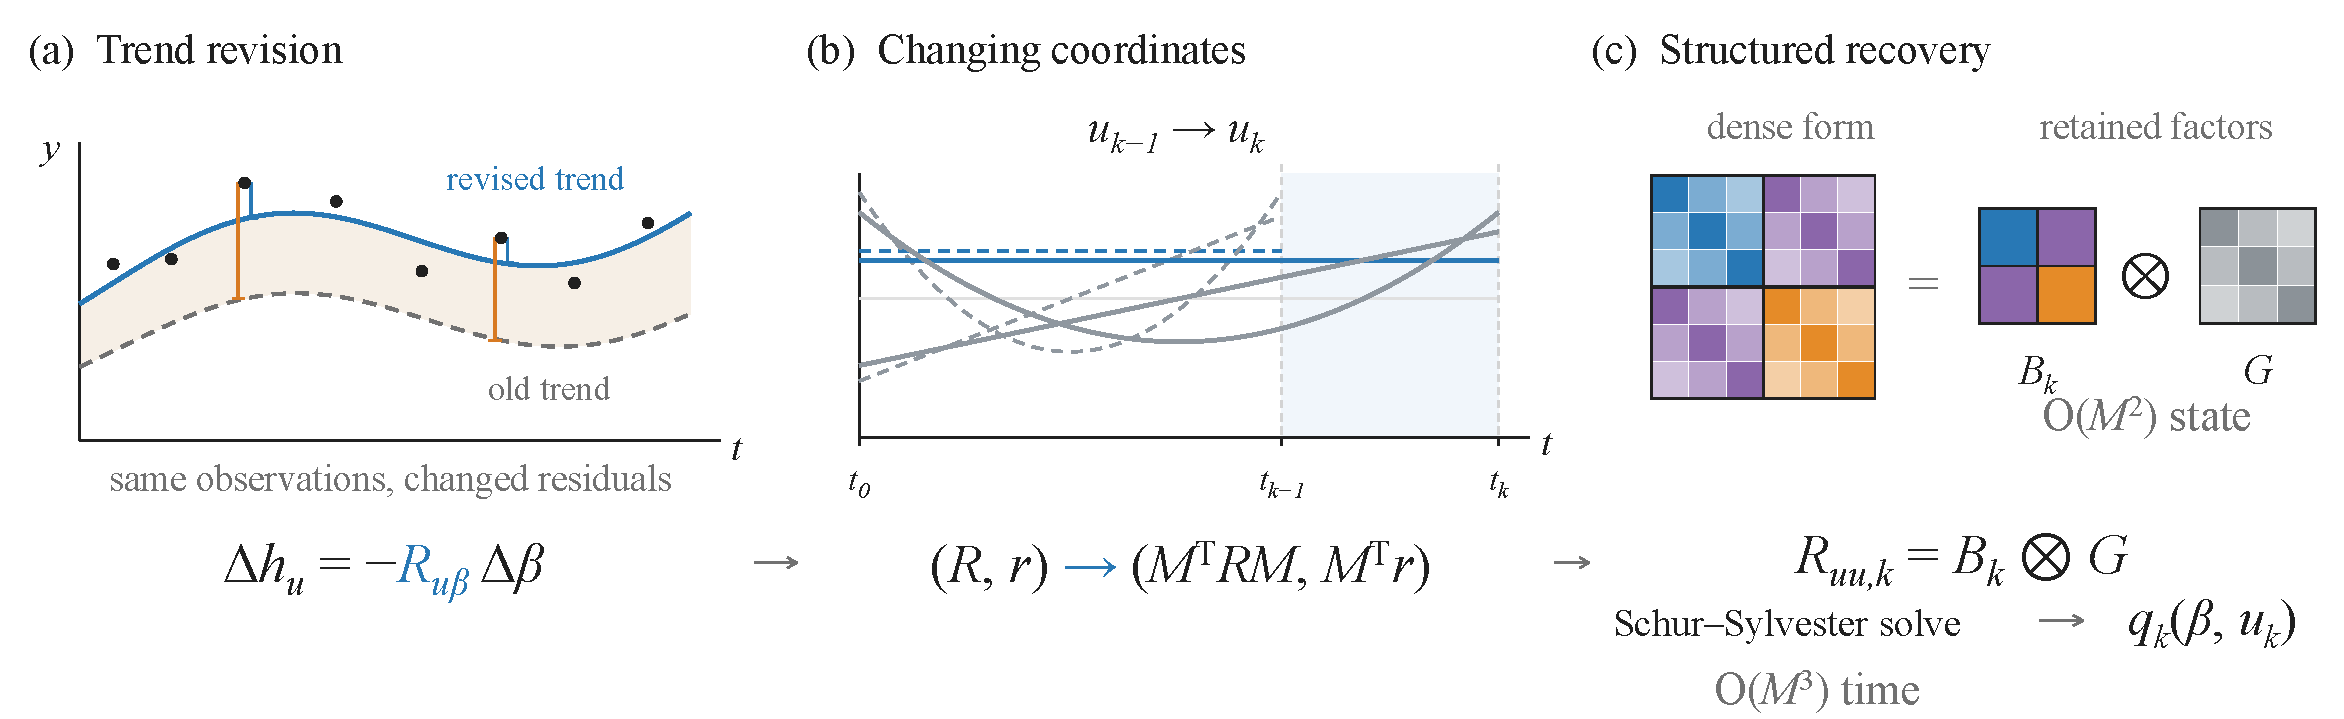
\includegraphics[width=\textwidth]{figures/Figure1_Publication_Overview_gap.pdf}
\par\vspace{-9pt} % Figure 1 only: compensate remaining artwork-to-caption gap.
\caption{Three stages of bounded-state inference. (a) Posterior trend revision changes the residual contribution of historical observations, making the retained trend--residual cross statistic necessary for replay-free correction. (b) Successive HiPPO states represent different GP functionals, so conditional projection transports historical likelihood evidence between changing coordinates. (c) The single-Kronecker likelihood invariant enables structured recovery of the transferred finite target without dense product-state factorisation. The complexity annotation assumes $M_s\asymp M_t=M$ and fixed $d_\beta$ under Proposition~\ref{prop:kron-invariant}.}
\label{fig:revision-aware-overview}
\end{figure*}

\subsection{Required statistics for bounded Bayesian revision}

A bounded memory cannot preserve all historical observations. Therefore, the first question is which statistics are necessary for future posterior revision.

Consider the joint finite state
\[
z=[\beta^{\trans},u^{\trans}]^{\trans}.
\]

For fixed inducing coordinates, the Gaussian likelihood contribution is summarised by the natural parameters. With design $J_j=[\Phi_j,A_j]$, the Gaussian variational factor at fixed hyperparameters has
\begin{align}
 \Lambda_k&=\Lambda_0+\sigma_y^{-2}\sum_{j\leq k}J_j^{\trans}J_j,&
 h_k&=h_0+\sigma_y^{-2}\sum_{j\leq k}J_j^{\trans}y_j.
 \label{eq:natural}
\end{align}
Thus fixed-coordinate sequential accumulation is identical to optimising the same finite VFE factor over concatenated blocks. The off-diagonal precision contains the trend--residual cross-precision block $R_{\beta u}$, equivalently $R_{u\beta}=R_{\beta u}^{\trans}$, with
$R_{u\beta}=\sigma_y^{-2}\sum_j A_j^{\trans}\Phi_j$.

This cross-information determines how historical residual evidence should be corrected after the posterior mean changes. If old residual evidence was formed using $\widehat\beta$, define
\[
 h_u^{<k}(\widehat\beta)=\sigma_y^{-2}\sum_{j<k}A_j^{\trans}(y_j-\Phi_j\widehat\beta).
\]
Then a revised estimate $\widehat\beta'=\widehat\beta+\Delta_\beta$ gives
\begin{equation}
 h_u^{<k}(\widehat\beta')-h_u^{<k}(\widehat\beta)
 =-R_{u\beta}^{<k}\Delta_\beta.
 \label{eq:stale}
\end{equation}
A residual-only summary is stale whenever the right-hand side is nonzero. Once the historical blocks have been discarded, the correction can be reconstructed only if the retained state encodes the action of $R_{u\beta}$. The cross block therefore records the historical information required to reinterpret the compressed residual statistic after the posterior mean estimate is revised.
\begin{proposition}[Necessity of revision information in bounded Bayesian memory]
\label{prop:cross-necessity}
Fix the historical designs and a reference coefficient $\beta_0$. Suppose a replay-free
summary, together with $h_u^{<k}(\beta_0)$, must recover
$h_u^{<k}(\beta_0+\Delta)$ without error for every admissible
$\Delta\in\mathbb R^{d_\beta}$. Then the summary must determine the linear map
$\Delta\mapsto R_{u\beta}^{<k}\Delta$; when the admissible changes span
$\mathbb R^{d_\beta}$, this determines $R_{u\beta}^{<k}$ itself. Hence retaining
$R_{u\beta}$, or an information-equivalent encoding of its action, is necessary
for faithful correction after arbitrary posterior trend revision.
\end{proposition}
This proposition establishes the first principle of evolving Bayesian memory: a finite state is not sufficient merely because it summarises the current posterior; it must also preserve the information required to reinterpret historical evidence after future model revision. Faithful replay-free revision therefore requires retaining $R_{u\beta}$, or an information-equivalent representation of its action. The proof is given in Appendix~\ref{app:cross-necessity}.

\subsection{Transporting Bayesian evidence between evolving representations}

The second challenge is that a bounded state may need to move between different coordinate systems. Successive HiPPO variables $u_o$ and $u_n$ have equal dimension but represent different GP functionals, and replacing one representation by the other need not be an invertible reparameterisation. We therefore project the historical log-likelihood factor into the current representation while keeping it separate from the prior expressed in the current coordinates. Write the retained historical factor as

\begin{equation}
 \widetilde{\ell}_o(\beta,u_o) \propto
 \exp\!\left\{ -\frac12 z_o^\trans R_o z_o+r_o^\trans z_o \right\}.
\label{eq:old-like}
\end{equation}

Let $L_{on}=K_{on}K_{nn}^{-1}$ denote the conditional-mean map from the new GP functionals to the old ones, and let $M_{on}=\operatorname{diag}(I,L_{on})$. Taking the conditional expectation of $\log \widetilde{\ell}_o(\beta,u_o)$ under $p(u_o\mid u_n)$ gives a quadratic log factor in $(\beta,u_n)$.
\begin{proposition}[Optimal projection of historical Bayesian evidence]
\label{prop:joint-transfer}
Define
\begin{equation}
 \log\widetilde\ell_{o\rightarrow n}(\beta,u_n)
 =\E_{p(u_o\mid u_n)}[\log\widetilde\ell_o(\beta,u_o)]+\mathrm{const},
 \label{eq:projection}
\end{equation}
where $K_{nn}\succ0$. Then the non-constant natural parameters are
\begin{equation}
 R_{o\rightarrow n}=M_{on}^{\trans}R_oM_{on},
 \qquad r_{o\rightarrow n}=M_{on}^{\trans}r_o.
 \label{eq:transfer}
\end{equation}
In particular, $R_{\beta u}\leftarrow R_{\beta u}L_{on}$ and
$R_{uu}\leftarrow L_{on}^{\trans}R_{uu}L_{on}$.
\end{proposition}
This transformation preserves the quadratic natural-parameter form required by the online recursion. Appendix~\ref{app:joint-transfer} gives the derivation. The projection is generally lossy because the new finite state need not retain all information represented by the old GP functionals; Section~4.3 quantifies this loss.

\subsection{Information loss under finite representation transfer}

A changing representation inevitably introduces information loss. The question is not whether loss occurs, but which part of historical evidence cannot be represented in the new finite state. Conditional expectation gives the $L^2$-optimal representation of the historical log factor among functions measurable in $(\beta,u_n)$, but the projection is not generally lossless. Components of the old log likelihood that are not measurable in $(\beta,u_n)$ cannot be represented after transfer. Proposition~\ref{prop:transfer-mse} quantifies this one-step loss.

Assume $K_{nn}\succ0$, $R_{uu}=R_{uu}^{\trans}$, and finite Gaussian second moments. Let
$\Sigma_{o\mid n}=K_{oo}-K_{on}K_{nn}^{-1}K_{no}$ and partition the old quadratic factor as in Eq.~(\ref{eq:old-like}).
\begin{proposition}[One-step projection optimality and loss]
\label{prop:transfer-mse}
For $g(\beta,u_o)=\log\widetilde\ell_o(\beta,u_o)$ up to an additive constant, $\E[g\mid\beta,u_n]$ is its optimal $L^2$ approximation measurable in $(\beta,u_n)$. With
\[
 a=r_u-R_{u\beta}\beta-R_{uu}L_{on}u_n,
\]
the conditional projection error is
\begin{equation}
\begin{aligned}
 &\E[(g-\E[g\mid\beta,u_n])^2\mid\beta,u_n] \\
 &=a^{\trans}\Sigma_{o\mid n}a
 +\tfrac12\operatorname{tr}[(R_{uu}\Sigma_{o\mid n})^2].
\end{aligned}
\label{eq:transfer-mse}
\end{equation}
\end{proposition}
The result is deliberately local: it characterises the best one-step representation in the new finite state and does not imply monotone or globally lossless repeated transfer. The proof, operator-norm bound, and nested-space corollary are given in Appendix~\ref{app:transfer-proof}.

\subsection{Structure-preserving transport}

The previous sections determine whether a finite Bayesian state can be correctly revised and transported. We now ask whether such a state remains computationally useful. Under a separable residual kernel and fixed spatial geometry, the coordinate change acts only on the temporal factor. With fixed spatial observations and inducing functionals, $C$ is constant and $G=C^{\trans}C$, while
$L_{k-1,k}=L_t\otimes I_{M_s}$ with
$L_t=K_{k-1,k}^{(t)}(K_{k,k}^{(t)})^{-1}$.

\begin{proposition}[Single-Kronecker likelihood invariant]
\label{prop:kron-invariant}
Assume a separable residual kernel, unchanged spatial inducing and observation functionals, Cartesian blocks, and homoscedastic Gaussian noise. If $R_{uu,k-1}=B_{k-1}\otimes G$, then conditional transport followed by assimilation gives
\begin{align}
 B_k&=L_t^{\trans}B_{k-1}L_t+\sigma_y^{-2}P_{t,k}^{\trans}P_{t,k}, \nonumber\\
 R_{uu,k}&=B_k\otimes G,
 \label{eq:kron-precision}
\end{align}
Starting from $B_0=0$, the invariant holds at every block.
\end{proposition}
The invariant is preserved by the interaction between the separable kernel and the restricted temporal coordinate transformation; it is not an additional dense factorisation assumption. The proof is in Appendix~\ref{app:kron-invariant}. Adding the prior produces the two-term residual posterior operator
\begin{equation}
D_u=K_{t,k}^{-1}\otimes K_s^{-1}+B_k\otimes G.
\label{eq:du-operator}
\end{equation}
The joint precision is
\begin{equation}
 \Lambda_k=
 \begin{bmatrix}A_\beta&B_{\beta u}\\B_{\beta u}^{\trans}&D_u\end{bmatrix}.
 \label{eq:joint-precision}
\end{equation}
The persistent state is $\{R_{\beta\beta,k},R_{\beta u,k},B_k,r_{\beta,k},H_{u,k},K_{t,k}\}$, together with fixed model quantities, where $r_{u,k}=\operatorname{vec}(H_{u,k})$. Proposition~4 reduces the persistent likelihood state to the temporal factor $B_k$, the fixed spatial factor $G$, and the mean--residual cross statistics; the dense $(M_sM_t)\times(M_sM_t)$ likelihood block is never materialised. The persistent-state dimension is therefore independent of stream length.

\subsection{Exact recovery of the projected Bayesian state}

The final question is whether efficient recovery introduces additional approximation beyond the finite representation transfer itself. Propositions 1--4 determine what historical information must be retained, how it is projected between changing coordinates, what finite projection can lose, and which separable structure survives. It remains to recover the resulting coupled Gaussian posterior without materialising the $M_sM_t$-dimensional residual precision. The standard Schur complement reduces joint recovery to applications of $D_u^{-1}$ and one $d_\beta$-dimensional solve. We therefore focus on the nontrivial residual solve, whose Kronecker structure admits the following matrix-equation form.

\begin{lemma}[Structured Sylvester solve of the residual block]
\label{lem:sylvester}
For symmetric positive-definite $K_s,K_{t,k}$ and positive-semidefinite $G,B_k$, the system
$D_u\operatorname{vec}(Z)=\operatorname{vec}(Q)$ is equivalent to
\begin{equation}
 K_s^{-1}ZK_{t,k}^{-1}+GZB_k=Q.
 \label{eq:sylvester}
\end{equation}
After whitening and separately diagonalising the spatial and temporal factors,
the matrix equation decouples elementwise,
\begin{equation}
 \widehat Z_{ij}=\frac{\widehat Q_{ij}}{1+\gamma_i\eta_j}.
 \label{eq:sylvester-solution}
\end{equation}
The transformations and recovery map are given in Appendix~\ref{app:sylvester-proof}.
\end{lemma}
Preserving the residual likelihood factorisation makes this classical matrix-equation solve applicable at every online update. The derivation and predictive covariance calculations are given in Appendix~\ref{app:sylvester-proof}.

\begin{theorem}[Equivalence to dense recovery of the transferred target]
\label{thm:dense-equivalence}
Under the assumptions of Proposition~\ref{prop:kron-invariant}, proper Gaussian priors, fixed hyperparameters, and declared numerical regularisation, the Schur-complement recovery together with Lemma~\ref{lem:sylvester} produces the same posterior means, covariance quadratic forms, and marginal predictive variances as densely solving the same precision $\Lambda_k$ in Eq.~(\ref{eq:joint-precision}), up to floating-point error and jitter.
\end{theorem}
The proof is in Appendix~\ref{app:dense-equivalence}. Theorem~\ref{thm:dense-equivalence} separates two sources of error: representation error caused by projecting historical evidence, and numerical error caused by solving the resulting Gaussian system. The Schur--Sylvester solver introduces no additional approximation beyond the finite representation transfer. For fixed mean dimension and balanced spatial and temporal budgets, recovery uses $O(M^3)$ time and $O(M^2)$ persistent memory; the general expressions are given in Appendix~\ref{app:complexity}.

\begin{table}[H]
\small
\setlength{\tabcolsep}{2pt}
\begin{tabularx}{\columnwidth}{@{}r@{\hspace{0.45em}}X@{}}
\toprule
\multicolumn{2}{@{}l}{\textbf{Algorithm 1} \method: replay-free update}\\
\midrule
\multicolumn{2}{@{}p{\columnwidth}@{}}{\textbf{Require:} stream $\mathcal D_{1:K}$ with $(V_k,Q_k)$; budgets $(M_s,M_t)$; prior $p(\beta)$.}\\[1pt]
1 & $\theta\leftarrow\textsc{Calibrate}(\mathcal D_1)$; $\textsc{Freeze}(\theta)$\\
2 & $\mathcal S\leftarrow\textsc{InitialiseBoundedState}()$\\
3 & \textbf{for} $k=2,\ldots,K$ \textbf{do}\\
4 & \quad Observe $y_k(V_k)$\\
5 & \quad $L_t\leftarrow\textsc{HiPPOTransfer}(\mathcal H_{k-1},\mathcal H_k;\theta)$\\
6 & \quad $\mathcal S\leftarrow\textsc{Assimilate}(\textsc{Transport}(\mathcal S,L_t),\mathcal D_k[V_k])$\\
7 & \quad $q_k(\beta,u_k)\leftarrow\textsc{SchurSylvester}(\mathcal S)$\\
8 & \quad $(\mu_k,v_k)\leftarrow\textsc{Predict}(q_k,Q_k)$ \quad {\scriptsize\itshape // before reading $y_k(Q_k)$}\\
9 & \textbf{end for}\\
\multicolumn{2}{@{}p{\columnwidth}@{}}{\textbf{Return:} predictions and bounded state $\mathcal S_K$.}\\
\bottomrule
\end{tabularx}
\end{table}
\FloatBarrier

Algorithm~1 exposes the execution order and strict-online information boundary;
Propositions~\ref{prop:joint-transfer}--\ref{prop:kron-invariant} and the
Schur--Sylvester solve define its core operations. Here $\mathcal S_k$ is the bounded persistent likelihood state
defined above, containing $R_{\beta\beta,k}$, $R_{\beta u,k}$, $B_k$,
$r_{\beta,k}$, $H_{u,k}$, and $K_{t,k}$.

\section{Experiments}
\setcounter{dbltopnumber}{1}

We organise the experiments around four questions motivated by the analysis: (i) does the full construction transfer across domains? (ii) does retaining joint trend--residual information matter in practice? (iii) must historical evidence be updated when the HiPPO representation changes, and how accurate is the resulting finite-state transfer? and (iv) does the preserved Kronecker structure translate into measurable computational savings?

Unless stated otherwise, all online experiments use the same information boundary:
visible locations are observed, held-out locations are predicted before their labels
are revealed, and previously processed blocks are never replayed. The main
comparison reports RMSE, CRPS, Gaussian NLPD, and ECE; protocols, coverage,
per-split results, and additional diagnostics are provided in the appendix.
Table~1 anchors the cross-domain predictive comparison. Figure~2 shows representative PEMS-BAY trajectories, while Figure~3 mirrors the three stages in Figure~1 with controlled checks of revision-aware coupling, coordinate-consistent transfer, and structured posterior recovery. Complete per-split, calibration, transfer-capacity, and solver statistics are reported in Appendix~B.

\paragraph{Baselines.}
We compare against streaming sparse GP methods, structured spatio-temporal and
multi-output GP models, and the task-aligned IGNNK neural kriging model on
PEMS-BAY. OHSVGP provides a comparison with existing HiPPO-based GP memory,
while Kron-STGP serves as our fixed-coordinate control. Method references are
given in Table~1, and Appendix~B.2 records the archived implementation provenance.

\begin{table*}[t]
\centering
\caption{Cross-domain strict-online spatial prediction (mean $\pm$ SD; five splits for ERA5-Land/COVID-19 and three for PEMS-BAY). Bold and underlined values denote the best and second-best comparable results; `--' indicates unavailable metrics. PEMS-BAY uses contemporaneous held-out-sensor prediction.}
\label{tab:cross-domain}
\small
\setlength{\tabcolsep}{4.5pt}
\setlength{\cmidrulewidth}{0.25pt}
\setlength{\cmidrulekern}{0.8em}
\begin{tabular}{lrrrr}
\toprule
Method & RMSE $\downarrow$ & CRPS $\downarrow$ & NLPD $\downarrow$ & ECE $\downarrow$ \\
\midrule
\multicolumn{5}{l}{\textit{ERA5-Land}} \\
OSGPR~\citep{Bui2017} & $0.9833{\pm}0.0127$ & $0.5612{\pm}0.0086$ & $1.5847{\pm}0.0294$ & $0.1131{\pm}0.0051$ \\
StreamingSGPR~\citep{Maddox2021} & $1.0660{\pm}0.0196$ & $0.6283{\pm}0.0144$ & $1.7331{\pm}0.0466$ & $0.1543{\pm}0.0080$ \\
OHSVGP~\citep{Chen2025} & $0.7303{\pm}0.0302$ & $0.4132{\pm}0.0170$ & $1.2989{\pm}0.0686$ & $\underline{0.1063{\pm}0.0091}$ \\
\addlinespace[2pt]\cmidrule(lr){1-5}\addlinespace[0.5pt]
Kron-STGP & $\underline{0.4166{\pm}0.0046}$ & $\underline{0.2391{\pm}0.0016}$ & $\underline{0.6590{\pm}0.0051}$ & $0.1711{\pm}0.0018$ \\
\method & $\mathbf{0.1416{\pm}0.0036}$ & $\mathbf{0.0766{\pm}0.0017}$ & $\mathbf{-0.3349{\pm}0.0434}$ & $\mathbf{0.0669{\pm}0.0067}$ \\
\midrule
\multicolumn{5}{l}{\textit{COVID-19}} \\
Persistence & $0.1955{\pm}0.0095$ & $0.1087{\pm}0.0051$ & $-0.1894{\pm}0.0321$ & $\underline{0.0656{\pm}0.0316}$ \\
Adaptive OSGPR~\citep{Bui2017} & $0.1742{\pm}0.0290$ & $0.0990{\pm}0.0167$ & $-0.2603{\pm}0.1757$ & $0.1267{\pm}0.0435$ \\
ST-SVGP~\citep{Hamelijnck2021} & $0.2094{\pm}0.0136$ & $0.1192{\pm}0.0067$ & $-0.0840{\pm}0.0390$ & $0.0900{\pm}0.0239$ \\
LMC-SVGP~\citep{Jeong2023} & $0.3376{\pm}0.0529$ & $0.1965{\pm}0.0281$ & $1.0809{\pm}0.4905$ & $0.1806{\pm}0.0140$ \\
ICM-SVGP~\citep{Jeong2023} & $0.3435{\pm}0.0447$ & $0.2002{\pm}0.0219$ & $1.0005{\pm}0.3588$ & $0.1797{\pm}0.0016$ \\
FSDE-SVI~\citep{Jeong2023} & $0.4705{\pm}0.0478$ & $0.2580{\pm}0.0158$ & $0.6693{\pm}0.1044$ & $\mathbf{0.0238{\pm}0.0066}$ \\
\addlinespace[2pt]\cmidrule(lr){1-5}\addlinespace[0.5pt]
Kron-STGP & $\underline{0.1605{\pm}0.0107}$ & $\underline{0.0922{\pm}0.0055}$ & $\underline{-0.3029{\pm}0.0533}$ & $0.1427{\pm}0.0240$ \\
\method & $\mathbf{0.1580{\pm}0.0120}$ & $\mathbf{0.0885{\pm}0.0058}$ & $\mathbf{-0.3621{\pm}0.0583}$ & $\underline{0.1183{\pm}0.0343}$ \\
\midrule
\multicolumn{5}{l}{\textit{PEMS-BAY}} \\
IGNNK~\citep{Wu2021IGNNK} & $\underline{0.7968{\pm}0.1226}$ & -- & -- & -- \\
OHSVGP & $0.8190{\pm}0.0681$ & $\underline{0.4064{\pm}0.0204}$ & $\underline{1.2312{\pm}0.0760}$ & $\underline{0.1671{\pm}0.0124}$ \\
OSGPR & $0.8207{\pm}0.0685$ & $0.4130{\pm}0.0211$ & $1.2318{\pm}0.0652$ & $0.1816{\pm}0.0083$ \\
\addlinespace[2pt]\cmidrule(lr){1-5}\addlinespace[0.5pt]
Kron-STGP & $0.8139{\pm}0.0695$ & $0.4104{\pm}0.0220$ & $1.2242{\pm}0.0664$ & $0.1827{\pm}0.0096$ \\
\method & $\mathbf{0.7666{\pm}0.0629}$ & $\mathbf{0.3774{\pm}0.0193}$ & $\mathbf{1.1883{\pm}0.1076}$ & $\mathbf{0.1317{\pm}0.0196}$ \\
\bottomrule
\end{tabular}
\end{table*}



\subsection{Cross-domain replay-free prediction}

We first test the same bounded-state inference construction across three
qualitatively different processes. ERA5-Land provides the longest
environmental stream and uses a comparatively rich meteorological mean
representation; COVID-19 introduces weekly public-health regime changes; and
PEMS-BAY tests urban mobility with a substantially simpler mean design.
PEMS-BAY is evaluated as contemporaneous held-out-sensor prediction rather
than standard future traffic forecasting, making IGNNK a task-aligned external
kriging baseline \citep{Li2018DCRNN,Wu2021IGNNK}. Together, the three settings
test portability of the inference construction rather than performance of one
domain-specific forecasting architecture.

\begin{figure}[t!]
\centering
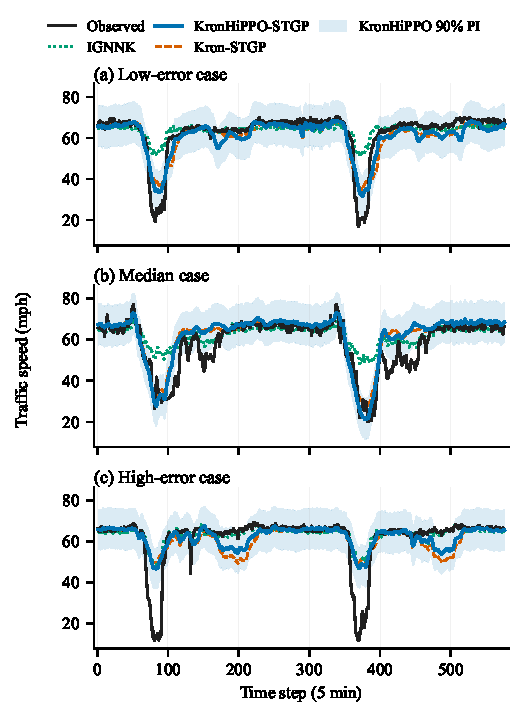
\includegraphics[width=\columnwidth]{figures/fig_representative_replay_free.pdf}
\caption{PEMS-BAY predictions across three predeclared difficulty regimes. The panels show seed-1 sensors nearest the 15th/50th/85th percentiles of KronHiPPO-STGP RMSE. Lines compare KronHiPPO-STGP with IGNNK and Kron-STGP; shading shows the 90\% predictive interval. Sensor IDs and selection details are reported in Appendix~B.}
\label{fig:representative-replay-free}
\end{figure}

Table~\ref{tab:cross-domain} shows consistent performance of the same replay-free construction across all three domains. \method attains the lowest mean RMSE and the lowest comparable CRPS and NLPD, although the calibration metrics do not produce a uniform ranking. The cross-domain pattern is therefore more informative than dominance on every individual metric. On PEMS-BAY, the improvement also persists outside the high-dimensional meteorological mean design used on ERA5 and against the task-aligned IGNNK baseline.

Figure~\ref{fig:representative-replay-free} provides a qualitative view across the three predeclared PEMS-BAY difficulty regimes. In these displayed trajectories, IGNNK smooths several abrupt congestion transitions that \method tracks more closely while also reporting predictive uncertainty. We treat these panels as illustrations rather than aggregate evidence; the quantitative comparison is reported in Table~\ref{tab:cross-domain}.

\subsection{Mechanism validation: memory and transfer}

\begin{figure*}[t]
\centering
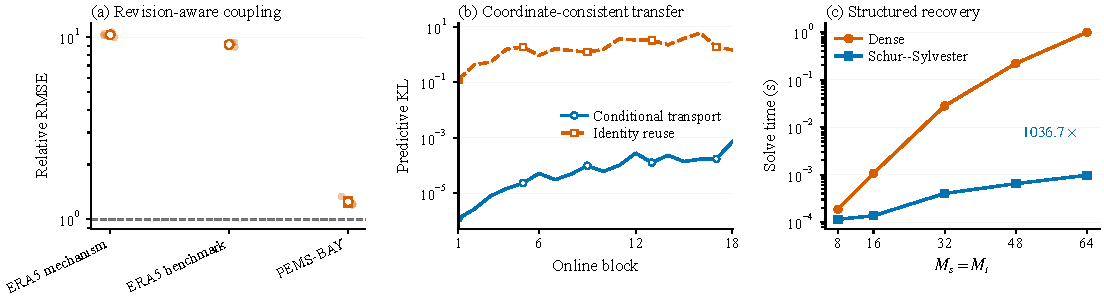
\includegraphics[width=\textwidth]{figures/figure3_main_mechanism.pdf}
\caption{Controlled checks aligned with the three stages of Figure~1. (a) Removing the trend--residual cross-precision block increases RMSE under two ERA5-Land operating points and on PEMS-BAY; points show the per-split ratio (\(\mathrm{RMSE}_{\mathrm{zero\text{-}cross}}/\mathrm{RMSE}_{\mathrm{joint}}\)) under changing HiPPO coordinates, with (1) denoting no change. (b) Conditional transport keeps the online predictive distribution close to the current-representation variational reference, whereas identity reuse produces a persistent mismatch. (c) Schur--Sylvester recovery solves the same Gaussian system increasingly faster than dense recovery as the balanced product-state dimension grows. Error bars in (a) and bands in (b) denote sample standard deviations over the corresponding matched splits. Detailed predictive and calibration metrics and selected solver timings are reported in Appendix~B.6.}
\label{fig:main-mechanism}
\end{figure*}

\paragraph{Revision-aware memory.}
Figure~\ref{fig:main-mechanism}(a) tests the practical role of the trend--residual cross-precision block identified in Proposition~\ref{prop:cross-necessity}. Within each setting, every joint/changing and zero-cross/changing pair uses the same spatial split, frozen hyperparameters, inducing-variable budgets, and changing-coordinate updates. Zero-cross removes the accumulated trend--residual cross block after the transported historical and current-block statistics have been combined; all other retained statistics and assimilation steps are unchanged. Removing this block increases RMSE at both ERA5 operating points and on PEMS-BAY. At the archived Table-1 ERA5 operating point, RMSE rises from $0.1416$ to $1.2921$, while the full arm reproduces the archived predictions to numerical precision. This operating-point replication shows that the effect is not specific to the spectral-mixture mechanism configuration. Because the intervention removes both historical and current-block cross-block contributions, it tests joint mean--residual likelihood coupling rather than historical trend revision in isolation. Complete predictive and calibration metrics are reported in Appendix Table~\ref{tab:mechanism_full}; calibration does not yield a uniform ordering.

\paragraph{Coordinate identity versus transfer.}
Figure~\ref{fig:main-mechanism}(b) tests whether equal-dimensional HiPPO states can be treated as the same GP representation. Identity reuse carries the historical approximate-likelihood natural parameters forward unchanged while updating the HiPPO inducing representation; the prior, current-block update, hyperparameters, and posterior solver are held fixed. At $M_t=128$, conditional transport gives predictive KL $1.26\times10^{-4}$ to the reference posterior recomputed in the current representation, whereas identity reuse gives $2.07$. The mismatch propagates to prediction: identity reuse raises RMSE from $0.0795$ to $0.2651$ and reduces Coverage90 from $0.982$ to $0.632$. CRPS and NLPD worsen in the same comparison, while ECE moves in the opposite direction, so we do not claim a uniform calibration ordering. Complete statistics are reported in Appendix Table~\ref{tab:coordinate_control}.

\paragraph{Transfer fidelity.}
The capacity sweep separates finite-projection error from coordinate mismatch. Conditional transport is non-monotone in $M_t$, but predictive KL falls to $3.67\times10^{-3}$ at $M_t=64$ and $1.26\times10^{-4}$ at $M_t=128$, whereas identity reuse remains near order one for $M_t\ge32$. Increasing temporal capacity alone therefore does not correct coordinate mismatch; at the operating capacity, conditional transport closely matches the current-representation finite-dimensional target. We do not infer a general convergence guarantee from this sweep. Appendix Fig.~\ref{fig:transfer_solver_diagnostics} reports the complete capacity diagnostic.

\subsection{Structured posterior computation and efficiency}

Figure~\ref{fig:main-mechanism}(c) tests the computational consequence of the preserved Kronecker structure. Dense and Schur--Sylvester recovery solve the same positive-definite systems with matched factors, right-hand sides, and BLAS threading. The mean paired speed-up rises from $7.9\times$ at $M_s=M_t=16$ to $1036.7\times$ at $M_s=M_t=64$, while relative solution error remains below $5\times10^{-12}$. For balanced budgets ($M_s=M_t=M$) and fixed $d_\beta$, the widening gap is consistent with the $O(M^3)$ structured and $O(M^6)$ dense solve complexities. Because both methods target the same Gaussian system, the speed-up is not obtained by changing the posterior approximation. Selected timings and relative errors are reported in Appendix Table~\ref{tab:solver}.

The matched solver benchmark is the evidence for the algorithmic claim. A separate archived RTX~4090 implementation audit includes full-model overhead: at $M_s=M_t=128$, KronHiPPO-STGP records $110.8\times$ lower training wall time and $8.8\times$ lower peak reserved memory than ST-SVGP, with $5.4\%$ higher RMSE. These are implementation-level measurements rather than architecture-neutral complexity ratios; the $40.4\times$ profiler-count difference is likewise implementation-specific. Appendix~B.7 reports the full audit and long-stream accounting.

\FloatBarrier

\FloatBarrier
\setcounter{dbltopnumber}{2}

\section{Conclusion}

We introduced \method, a bounded-memory variational GP method for jointly updating a parametric mean and spatio-temporal GP residual without replay. Across environmental, public-health, and traffic streams, the method provides strong point and probabilistic predictions while keeping persistent memory independent of stream length. The analysis and controlled experiments examine each component of the construction: retaining the joint information needed to revise past evidence, updating that evidence when the HiPPO representation changes, and preserving Kronecker structure for efficient posterior computation.

The current construction assumes separable residual kernels, fixed spatial
inducing and observation geometry, Cartesian-product observation blocks with
Gaussian likelihood, and frozen streaming hyperparameters;
richer observation patterns and likelihoods will require more general structured
states. The results also indicate that, in online probabilistic models, a changing
finite memory should be treated as a changing coordinate system for historical
evidence rather than as an interchangeable latent state.

\subsection*{AI use statement}

We used OpenAI ChatGPT and Codex as research-support and editing tools. Their use included suggesting literature-search queries and organising candidate sources; assisting with revisions to experimental code and additions to training scripts; organising experiment records and checking the consistency of tables and reported results; improving LaTeX layout, cross-references, and figure and table formatting; and suggesting language and structural revisions to selected sections. Generative-AI outputs were treated as suggestions rather than scholarly evidence. The authors checked cited claims against the original publications, reviewed and tested code changes, generated the reported numerical results by running the documented experiments, and verified mathematical arguments and reported values against project records. All material was selected, revised, and approved by the authors, who remain responsible for its accuracy and originality.

\bibliography{references}
\bibliographystyle{apalike}

\clearpage
\appendix
\thispagestyle{empty}
\onecolumn
\aistatstitle{KronHiPPO-STGP: Online Bayesian Spatio-temporal Modelling with Evolving Memory: Supplementary Materials}
\setcounter{table}{4}
\section*{Reproducibility statement}
The appendix specifies the information boundary, data splits, objectives, hyperparameter-freezing rule, metrics, and structured-solver check. The anonymised supplementary package contains machine-readable aggregate and per-seed mechanism results, the suite manifest, proof audit, and scripts used to run and visualise the diagnostics.

\subsection*{Ethics statement}
The study uses environmental observations and aggregate public-health data from public sources. It does not recruit participants, conduct clinical interventions, or access identifiable or individual-level health records. The models were evaluated as research methods and were not deployed for clinical or public-health decision making. Any operational use would require separate assessment of calibration, distribution shift, fairness, and the consequences of missed or false alarms.

\section{Derivations and exactness boundary}

\subsection{Proof of Proposition 1: necessity of the cross statistic}
\label{app:cross-necessity}

Let $S$ denote the retained summary and assume a zero-error decoder
$D(S,h_u(\beta_0),\Delta)=h_u(\beta_0+\Delta)$ for every admissible
$\Delta$. Equation~(\ref{eq:stale}) then implies
\[
 h_u(\beta_0)-D(S,h_u(\beta_0),\Delta)=R_{u\beta}\Delta.
\]
The retained information therefore determines the action of $R_{u\beta}$ on the
span of admissible changes. If this span is $\mathbb R^{d_\beta}$, evaluating
the decoder on a basis recovers every column of $R_{u\beta}$. Conversely,
retaining $R_{u\beta}$ makes the correction explicit through
Eq.~(\ref{eq:stale}). Two historical datasets with the same retained summary
but different actions $R_{u\beta}\Delta$ would require the decoder to return
different values from identical inputs, contradicting error-free recovery.

\subsection{Proof of Proposition 2: historical likelihood-factor transfer}
\label{app:joint-transfer}

Conditionally write $u_o=L_{on}u_n+\delta$ with $\E[\delta\mid u_n]=0$. For $z_o=M_{on}z_n+[0,\delta]^{\trans}$, substitution into Eq.~(\ref{eq:old-like}) followed by conditional expectation gives
\[
 -\tfrac12 z_n^{\trans}M_{on}^{\trans}R_oM_{on}z_n
 +r_o^{\trans}M_{on}z_n
 -\tfrac12\operatorname{tr}(R_{uu,o}\operatorname{Cov}(\delta)).
\]
The trace is constant in $(\beta,u_n)$, leaving Eq.~(\ref{eq:transfer}). The transferred cross block is therefore $R_{\beta u,o}L_{on}$. This establishes a one-step projected log factor and does not compare the resulting posterior with a full-history posterior expressed in the current inducing representation.

\subsection{Proof of Proposition 3: one-step projection optimality and loss}
\label{app:transfer-proof}

Write $u_o=m+\delta$, where $m=L_{on}u_n$ and, conditional on $(\beta,u_n)$, $\delta\sim\mathcal N(0,\Sigma_{o\mid n})$. Expanding the terms that depend on $\delta$ gives
\begin{align*}
 g(\beta,m+\delta)&=c(\beta,u_n)+a^{\trans}\delta
 -\tfrac12\delta^{\trans}R_{uu}\delta,\\
 a&=r_u-R_{u\beta}\beta-R_{uu}m.
\end{align*}
After centring,
\[
 g-\E[g\mid\beta,u_n]
 =a^{\trans}\delta-\tfrac12\{\delta^{\trans}R_{uu}\delta-
 \operatorname{tr}(R_{uu}\Sigma_{o\mid n})\}.
\]
The cross covariance vanishes because centred Gaussian third moments are zero. The linear term has variance $a^{\trans}\Sigma_{o\mid n}a$, while the unscaled quadratic term has variance $2\operatorname{tr}[(R_{uu}\Sigma_{o\mid n})^2]$. This gives Eq.~(\ref{eq:transfer-mse}), and optimality follows because conditional expectation is the orthogonal projection in $L^2$. Finally,
$a^{\trans}\Sigma a\leq\|\Sigma\|_2\|a\|_2^2$ and
$\operatorname{tr}[(R\Sigma)^2]=\|\Sigma^{1/2}R\Sigma^{1/2}\|_F^2\leq\|R\|_F^2\|\Sigma\|_2^2$.

For the nested-space statement, the conditional mean is again an $L^2$ projection. Its squared reconstruction error is the trace of the conditional covariance, and the Pythagorean theorem for nested projection subspaces makes this error non-increasing. This statement requires both the old target and its joint law to remain fixed; unrelated feature families at different $M_t$ need not be nested.

\subsection{Proof of Proposition 4: single-Kronecker likelihood invariant}
\label{app:kron-invariant}

Under separability and unchanged spatial functionals,
$K_{k-1,k}=K_{k-1,k}^{(t)}\otimes K_s$ and
$K_{k,k}=K_{k,k}^{(t)}\otimes K_s$. Hence
\begin{align*}
L_{k-1,k}&=K_{k-1,k}K_{k,k}^{-1}\\
&=\{K_{k-1,k}^{(t)}(K_{k,k}^{(t)})^{-1}\}\otimes I_{M_s}\\
&=L_t\otimes I_{M_s}.
\end{align*}
If $R_{uu,k-1}=B_{k-1}\otimes G$, conditional transport gives
\[
(L_t\otimes I)^{\trans}(B_{k-1}\otimes G)(L_t\otimes I)
=(L_t^{\trans}B_{k-1}L_t)\otimes G.
\]
For a Cartesian block, $A_k=P_{t,k}\otimes C$ and therefore
\[
\sigma_y^{-2}A_k^{\trans}A_k
=(\sigma_y^{-2}P_{t,k}^{\trans}P_{t,k})\otimes(C^{\trans}C).
\]
With $G=C^{\trans}C$, their sum is precisely $B_k\otimes G$. The base case
$B_0=0$, followed by induction over blocks, establishes Proposition~\ref{prop:kron-invariant}.

\subsection{Proof of Lemma 1: structured Sylvester solve for the inducing-variable precision block}
\label{app:sylvester-proof}

Under the column-major vectorisation convention,
$(A\otimes B)\operatorname{vec}(Z)=\operatorname{vec}(BZA^{\trans})$.
Applying this identity to the two terms in Eq.~(\ref{eq:du-operator}) gives
Eq.~(\ref{eq:sylvester}). Substitute

\begin{equation*}
 Z=K_s^{1/2}\widetilde ZK_{t,k}^{1/2}
\end{equation*}

and multiply by the corresponding square roots. This gives
\begin{align*}
\widetilde Z+\widetilde G\,\widetilde Z\,\widetilde B&=\widetilde Q,
\end{align*}
where
\begin{equation*}
\begin{aligned}
\widetilde G&=K_s^{1/2}GK_s^{1/2},\qquad
\widetilde B=K_{t,k}^{1/2}B_kK_{t,k}^{1/2},\\
\widetilde Q&=K_s^{1/2}QK_{t,k}^{1/2}.
\end{aligned}
\end{equation*}
Let
\[
\widetilde G=U_s\operatorname{diag}(\gamma_i)U_s^{\trans},\qquad
\widetilde B=U_t\operatorname{diag}(\eta_j)U_t^{\trans},
\]
and define
\[
\widehat Z=U_s^{\trans}\widetilde ZU_t,\qquad
\widehat Q=U_s^{\trans}\widetilde Q U_t.
\]
Writing $\widetilde Z=U_s\widehat ZU_t^{\trans}$ and rotating by these
eigensystems gives
$(1+\gamma_i\eta_j)\widehat Z_{ij}=\widehat Q_{ij}$.
Positive semidefiniteness implies $1+\gamma_i\eta_j\geq1$, establishing
Eq.~(\ref{eq:sylvester-solution}) and uniqueness. The recovered matrix is
$\widetilde Z=U_s\widehat ZU_t^{\trans}$ followed by
$Z=K_s^{1/2}\widetilde ZK_{t,k}^{1/2}$.

\subsection{Proof of Theorem 1: dense equivalence of the transferred finite-dimensional target}
\label{app:dense-equivalence}

Proposition~\ref{prop:kron-invariant} gives the lower-right block
$D_u$ of the densely assembled transferred precision. Lemma~\ref{lem:sylvester}
replaces each application of $D_u^{-1}$ with an algebraically equivalent structured matrix
solve, after which the standard Schur-complement block inverse is applied to the
same $\Lambda_k$. Define the Schur complement
\[
P_\beta=A_\beta-B_{\beta u}D_u^{-1}B_{\beta u}^{\trans}.
\]
Then
\[
S_{\beta\beta}=P_\beta^{-1},\qquad
S_{\beta u}=-P_\beta^{-1}B_{\beta u}D_u^{-1},
\]
\[
S_{uu}=D_u^{-1}+D_u^{-1}B_{\beta u}^{\trans}
P_\beta^{-1}B_{\beta u}D_u^{-1}.
\]
These are precisely the blocks of $\Lambda_k^{-1}$, so the posterior means and
covariance quadratic forms agree with the dense posterior solve. Adding the same full-GP
conditional residual to both predictive variances preserves this equality. Any
remaining difference arises only from finite-precision arithmetic and the same
declared jitter; the structured solve introduces no additional posterior approximation.

\subsection{Prediction with the full conditional}

Let $a_*$ denote the conditional-mean projection row, $h_*=[\phi_*^{\trans},a_*^{\trans}]^{\trans}$, and let $S_k$ be the joint variational covariance. The predictive moments are
\begin{align}
 \E[y_*]&=\phi_*^{\trans}m_\beta+a_*^{\trans}m_u,\\
 \operatorname{Var}(y_*)&=\sigma_y^2+h_*^{\trans}S_kh_*+\nu_*,
 \qquad
 \nu_*=k_{**}-a_*^{\trans}K_ua_*.
\end{align}
The $\nu_*$ term is the GP conditional variance term and is distinct from the VFE trace correction used during hyperparameter calibration.

\subsection{Detailed posterior-solve cost}
\label{app:complexity}
A dense inducing-variable precision factorisation costs $O(M_s^3M_t^3)$ time and
$O(M_s^2M_t^2)$ memory. Accounting for the $d_\beta$ cross-block right-hand
sides and the Schur complement, structured posterior solve costs
\begin{multline}
 O\!\left(M_s^3+M_t^3+(d_\beta+1)
 (M_s^2M_t+M_sM_t^2)\right.\\
 \left.{}+d_\beta^2M_sM_t+d_\beta^3\right),
 \label{eq:recovery-cost}
\end{multline}
and the persistent state occupies
\begin{equation}
 O(M_s^2+M_t^2+(d_\beta+1)M_sM_t+d_\beta^2),
 \label{eq:state-cost}
\end{equation}
for fixed budgets, independently of the number of elapsed blocks. These expressions
cover core posterior computation and persistent state, and exclude current-block
statistic formation, data loading, Task-1 calibration, and all-point prediction.

\section{Experimental protocols}

\subsection{Evaluation metrics}

For $N$ held-out predictions with Gaussian posterior
$y_i\sim\mathcal N(\mu_i,\sigma_i^2)$, define
$z_i=(y_i-\mu_i)/\sigma_i$.  We report
\begin{align}
\operatorname{RMSE}
&=\left[\frac{1}{N}\sum_{i=1}^{N}(y_i-\mu_i)^2\right]^{1/2},
\\
\operatorname{NLPD}
&=\frac{1}{N}\sum_{i=1}^{N}
\left[\frac{1}{2}\log(2\pi\sigma_i^2)
+\frac{(y_i-\mu_i)^2}{2\sigma_i^2}\right],
\\
\operatorname{CRPS}_i
&=\sigma_i\left[z_i\{2\Phi(z_i)-1\}
+2\phi(z_i)-\frac{1}{\sqrt{\pi}}\right],
\\
\operatorname{CRPS}
&=\frac{1}{N}\sum_{i=1}^{N}\operatorname{CRPS}_i,
\end{align}
where $\Phi$ and $\phi$ denote the standard-normal distribution and density.
Calibration is measured over the central predictive intervals
$\mathcal A=\{0.05,0.15,\ldots,0.95\}$:
\begin{align}
\widehat C(\alpha)
&=\frac{1}{N}\sum_{i=1}^{N}
\mathbf{1}\!\left(
|y_i-\mu_i|\leq
\Phi^{-1}\!\left(\frac{1+\alpha}{2}\right)\sigma_i
\right),
\\
\operatorname{ECE}
&=\frac{1}{|\mathcal A|}\sum_{\alpha\in\mathcal A}
|\widehat C(\alpha)-\alpha|.
\end{align}
All four metrics are lower-is-better.  Tables report the mean and sample
standard deviation across the archived spatial splits.  For archived
sample-based predictive distributions, the same central-interval definition
is evaluated using empirical predictive quantiles.

For the ERA5-Land and PEMS-BAY mechanism suites, complete mean $\pm$ sample
SD results, including Coverage90, are reported in Appendix Table~\ref{tab:mechanism_full}.

\FloatBarrier
\subsection{Dataset and protocol overview}

Table~\ref{app:dataset-overview} summarises the spatial units, temporal stream,
information boundary, and role of each dataset. Dataset-specific figures are
shown in the corresponding sections to keep each visual legible at print size.

\begin{table}[H]
\centering
\caption{Dataset and strict-online protocol overview.}
\label{app:dataset-overview}
\scriptsize
\setlength{\tabcolsep}{0.7pt}
\begin{tabular}{@{}lllll@{}}
\toprule
Dataset & Units & Stream & V / H & Domain \\
\midrule
ERA5-Land & 1,000 UK & 171 blk. & 800/200 & Environmental \\
COVID & 52 juris. & 143 wk. & 42/10 & Public health \\
PEMS & 325 sens. & 5-min & 260/65 & Traffic \\
\bottomrule
\end{tabular}
\end{table}
\FloatBarrier

\paragraph{Baseline implementations.}
Table~1 compares streaming sparse GP methods, structured spatio-temporal and multi-output GP baselines, OHSVGP as an existing HiPPO-based GP method, and IGNNK as the task-aligned neural kriging baseline. The provenance table below includes only information recoverable from the archived code, manifests, and result records; unavailable fields are marked as not recorded. OSGPR and Adaptive OSGPR use the same official \texttt{OSGPR\_VFE} core but differ in their archived update policies. StreamingSGPR denotes the same \texttt{online\_gp} implementation used in Table~1 and Appendix Table~\ref{app:efficiency-online}.

\begin{table}[H]
\centering
{\small\bfseries Archived baseline implementation provenance: implementation and objective.}\par\smallskip
\small
\setlength{\tabcolsep}{5pt}
\renewcommand{\arraystretch}{1.18}
\begin{tabularx}{\textwidth}{@{}>{\raggedright\arraybackslash}p{0.16\textwidth}>{\raggedright\arraybackslash}p{0.53\textwidth}>{\raggedright\arraybackslash}X@{}}
\toprule
Method & Implementation & Objective \\
\midrule
OSGPR & Official \texttt{OSGPR\_VFE} \citep{Bui2017} & Streamed VFE log factor \\
Adaptive OSGPR & Same official core; adaptive wrapper & VFE with causal parameter updates \\
StreamingSGPR & Official \texttt{online\_gp} code path \citep{Maddox2021} & Fantasy-model conditioning \\
OHSVGP & Official \texttt{HIPPOSVGP} multidimensional model \citep{Chen2025} & Online variational HiPPO GP \\
ST-SVGP & Archived causal-refit adapter \citep{Hamelijnck2021} & Gaussian ELBO \\
LMC-SVGP & FactorialSDE LMC constructor \citep{Jeong2023}; GPflow SVGP \citep{Hensman2015} & Gaussian SVGP ELBO \\
ICM-SVGP & FactorialSDE intrinsic-coregionalisation constructor (archive id \texttt{imc\_svgp}) \citep{Jeong2023}; GPflow SVGP \citep{Hensman2015} & Gaussian SVGP ELBO \\
FSDE-SVI & FactorialSDE implementation \citep{Jeong2023} & State-space variational ELBO \\
IGNNK & Official \texttt{basic\_structure.IGNNK} \citep{Wu2021IGNNK} & Masked-node MSE \\
\bottomrule
\end{tabularx}
\end{table}

\begin{table}[H]
\centering
{\small\bfseries Archived baseline implementation provenance: budgets, inputs, and calibration.}\par\smallskip
\small
\setlength{\tabcolsep}{4pt}
\renewcommand{\arraystretch}{1.18}
\begin{tabularx}{\textwidth}{@{}>{\raggedright\arraybackslash}p{0.16\textwidth}>{\raggedright\arraybackslash}p{0.22\textwidth}>{\raggedright\arraybackslash}p{0.30\textwidth}>{\raggedright\arraybackslash}X@{}}
\toprule
Method & Inducing/state budget & Mean/covariates & Calibration \\
\midrule
OSGPR & ERA5: $2{\times}64$; PEMS: $4{\times}32$ & Task-1-fitted residual offset & Task-1 kernel/noise frozen \\
Adaptive OSGPR & COVID: $8{\times}32=256$ & Archived Task-1 offset & 25 Task-1 steps/block; 5 online steps \\
StreamingSGPR & ERA5: $2{\times}64=128$ & Task-1-fitted residual offset & Task-1 kernel/noise frozen; 20\% resampling \\
OHSVGP & ERA5: $M=32$, 128 RFF; PEMS: $M=64$, 256 RFF & Task-1-fitted residual offset & Task-1 kernel/noise mapped and frozen; variational state updated online \\
ST-SVGP & COVID: 32 spatial inducing points & Target series only & Task-1 fit; causal weekly refits \\
LMC-SVGP & not recorded for the reported three-run aggregate & Target series only & not recorded in returned aggregate \\
ICM-SVGP & not recorded for the reported three-run aggregate & Target series only & not recorded in returned aggregate \\
FSDE-SVI & not recorded for the reported three-run aggregate & Target series only & not recorded in returned aggregate \\
IGNNK & hidden width 100; diffusion order 1; 24-step window & Visible speeds, lagged held-out speeds, and fixed road graph & Task-1-only training; validation every 25 epochs \\
\bottomrule
\end{tabularx}
\end{table}

\subsection{ERA5-Land}

The processed dataset contains 2-m dew-point temperature and associated meteorological covariates from the ERA5-Land hourly product \citep{MunozSabater2019,MunozSabater2021} at 1,000 UK locations. Five paired spatial splits contain 800 visible and 200 held-out locations. Within each split, the validation locations used during Task-1 calibration are drawn from the visible set and remain disjoint from the 200 held-out evaluation locations. The mean design contains seven deterministic time-coordinate features and 126 current, lagged, and difference features from six non-target meteorological variables; the target itself is not used as an X-lag input. In the benchmark archive, OSGPR, StreamingSGPR, and OHSVGP receive deterministic Task-1-fitted mean offsets constructed from this feature design, whereas Kron-STGP and KronHiPPO-STGP retain the same features within their joint mean update. Both ERA5 configurations use the 186 Task-1 timestamps for VFE calibration. The scored stream begins at block 0 of Task 2 and contains 171 blocks across Tasks 2--10. The benchmark configuration uses the default temporal kernel, with at most 250 calibration iterations, validation every five iterations, and patience eight. The mechanism configuration uses a three-component spectral-mixture temporal kernel with 100 fixed calibration iterations. Both use $M_s=M_t=128$ and 256 random Fourier features. The archive names \texttt{task1\_10} and \texttt{task1\_2} refer to experiment configurations rather than the temporal extent of the calibration input. The joint posterior state, including $q_k(\beta)$, is updated blockwise.

The default protocol is contemporaneous spatial nowcasting. At each block, the 800 visible targets are assimilated before predictions are made at the 200 held-out locations. Historical raw observations are not revisited. Whole-field future forecasting, in which no current target is visible, is outside the scope of the present evidence and is not included in the main comparison.

\begin{figure}[tbp]
\centering
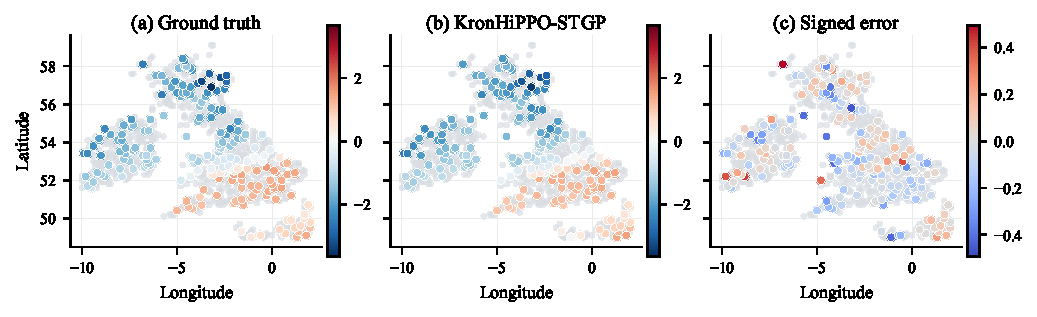
\includegraphics[width=0.98\textwidth]{figures/era5_long_tasks1_10_spatial_snapshot_horizontal.pdf}
\caption{ERA5-Land Tasks~1--10 long-stream spatial snapshot at the final online
block for the predeclared seed-0 split. The panels show the standardized target
field, the \method posterior mean, and the signed prediction error at the 200
held-out UK locations; the remaining 800 visible locations are shown in light
gray for spatial context. The map geometry is used only for visualisation.}
\label{app:era5-long-map}
\end{figure}
\FloatBarrier

\subsection{COVID-19}

The COVID-19 dataset contains 52 weekly jurisdiction-level hospital-admission series from the CDC NHSN Hospital Respiratory Data release \citep{CDCWeeklyHospitalization}. The target is the standardised $\log(1+x)$ transform of weekly confirmed COVID-19 admissions per 100,000 population.
Task~1 provides the initial 52-week calibration period, followed by 143 weeks
processed strictly online. Each formal split observes 42
jurisdictions and predicts 10 held-out jurisdictions before their labels are
revealed. The composite figure uses the predeclared seed-5 Connecticut and
Nevada trajectories, selected by the largest distance between z-scored
observed trajectories among the four archived candidates.

\begin{figure}[!t]
\centering
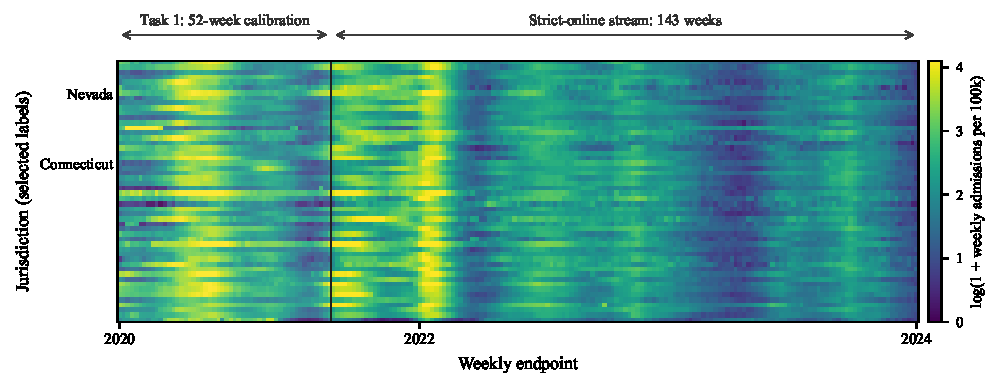
\includegraphics[width=0.96\textwidth]{figures/dataset_overview_covid_heatmap.pdf}
\vspace{3pt}

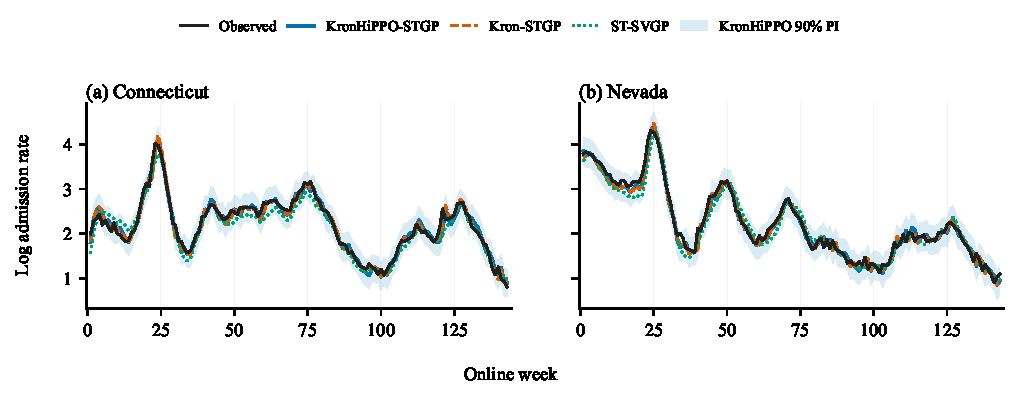
\includegraphics[width=0.96\textwidth]{figures/fig_covid_trajectories_side_by_side.pdf}
\caption{COVID-19 dataset structure and replay-free qualitative evidence. The
upper panel shows the jurisdiction-by-week overview, with the 52-week calibration
period separated from the subsequent 143-week strict-online stream. The lower
panels show seed-5 Connecticut and Nevada trajectories selected by the archived
observed-trajectory diversity rule; a shared y-scale and legend are used for the
same predictive methods in both jurisdictions.}
\label{app:covid-composite}
\end{figure}

\FloatBarrier

\subsection{PEMS-BAY}

PEMS-BAY contains traffic-speed measurements from 325 Bay Area sensors sampled every five minutes in the public DCRNN benchmark release \citep{Li2018DCRNN}. We use the
data for contemporaneous spatial nowcasting rather than future traffic
forecasting. In each formal split, 260 sensors are visible and 65 are held out,
with held-out labels revealed only after prediction. The protocol uses
$M_s=32$, $M_t=128$, 512 random Fourier features, and the locked road-context
X-lag mean design. All nine matched mechanism runs complete without OOM or
divergence.
Figure~\ref{fig:representative-replay-free} uses the predeclared seed-1 sensors
nearest the 15th, 50th, and 85th percentiles of full-stream \method RMSE:
sensors 400952, 400965, and 400178, respectively. Sensor selection therefore
follows the predefined \method difficulty quantiles. The common 48-hour plotting
window is selected independently using observed speeds only, by maximising the
median held-out speed range; the relative performance of the displayed methods
is not used for window selection.

\begin{figure}[!t]
\centering
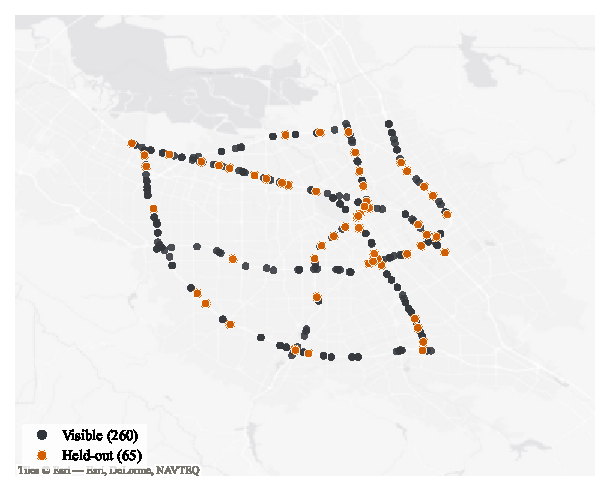
\includegraphics[width=0.78\textwidth]{figures/dataset_overview_pems.pdf}
\caption{PEMS-BAY sensor geometry for the archived seed-0 spatial split.
Dark-gray points are visible sensors and orange points are held-out sensors,
shown over a pale Bay Area road basemap. The geometry is used only to
visualise the contemporaneous held-out-sensor protocol. Map attribution is
included in the artwork.}
\label{app:pems-map}
\end{figure}

\subsection{Mechanism and transfer diagnostics}

Within each dataset, the joint/changing and zero-cross/changing variants share the same split, calibration, inducing-variable budgets, and changing inducing-representation maps. Zero-cross removes the accumulated trend--residual likelihood cross block after the transported historical and current-block statistics are combined. Joint/fixed-global uses complete-horizon temporal inducing representations and is reported separately as an offline representation reference.

The transfer diagnostic evaluates a separate mechanism by comparing the transported online state with a finite-dimensional variational reference posterior recomputed from the observed history in the current inducing representation. We report the marginal predictive Gaussian KL $\mathrm{KL}(p_{\mathrm{online}}\|p_{\mathrm{reference}})$, averaged first over query locations within each non-warm-up block, then over blocks within each seed, and finally across seeds. At $M_t=128$, the reported value $1.27\times10^{-4}$ is this aggregated diagonal predictive KL; it is neither a joint-output KL nor a solver residual. The solver benchmark instead uses identical positive-definite systems and right-hand sides for dense and structured posterior solves, thereby isolating numerical solution from representation transfer.

For each solver size, dense and structured posterior solves are evaluated on the same matched random systems. The displayed dense and structured runtimes are means, whereas speed-up is computed within each replicate as $t_{\mathrm{dense}}/t_{\mathrm{structured}}$ before averaging across replicates. The resulting mean speed-up therefore need not equal the ratio of the two displayed mean runtimes.
Figure~\ref{fig:main-mechanism} (c) visualises this matched solver benchmark, while Table~\ref{tab:solver} reports selected runtimes, paired speed-ups, and relative solution errors.

The lower off-diagonal block is reconstructed as the transpose when assembling the symmetric precision; all other retained statistics and assimilation steps remain unchanged. Because the removed block contains both historical and current-block contributions, the ablation tests joint likelihood coupling rather than historical trend revision alone.

Operating-point robustness. We repeat the zero-cross intervention under the archived ERA5 setting used in Table~1, without retuning either arm, to test whether the result depends on the spectral-mixture mechanism configuration. The full run reproduces the archived predictive means and variances to numerical precision (maximum absolute differences $4.23\times10^{-12}$ and $5.15\times10^{-15}$), while zero-cross again degrades every point and proper scoring-rule metric. Complete results are reported in Table~\ref{tab:mechanism_full}.

\begin{center}
\captionof{table}{Full mechanism results and ERA5 operating-point robustness check (mean $\pm$ sample SD). The first two blocks report the formal ERA5-Land and PEMS-BAY mechanism suites; the final block repeats the joint-versus-zero-cross intervention under the Table-1 ERA5 configuration. Coverage90 provides an additional calibration diagnostic.}
\label{tab:mechanism_full}
\small
\setlength{\tabcolsep}{4.0pt}
\begin{tabular}{@{}lrrrrr@{}}
\toprule
Variant & RMSE $\downarrow$ & CRPS $\downarrow$ & NLPD $\downarrow$ & ECE $\downarrow$ & Coverage90 \\
\midrule
\multicolumn{6}{@{}l}{\textit{ERA5-Land (five 171-block runs)}} \\
Joint / changing & $0.1251\pm0.0034$ & $0.0665\pm0.0014$ & $-0.6837\pm0.0186$ & $0.0461\pm0.0029$ & $0.9134\pm0.0035$ \\
Zero-cross / changing & $1.2898\pm0.0120$ & $0.9951\pm0.0088$ & $52.8139\pm1.9682$ & $0.6905\pm0.0018$ & $0.1148\pm0.0019$ \\
Joint / fixed-global & $0.1950\pm0.0030$ & $0.1420\pm0.0009$ & $0.2580\pm0.0043$ & $0.1807\pm0.0012$ & $0.9933\pm0.0006$ \\
\addlinespace[1pt]
\cmidrule(lr){1-6}
\addlinespace[1pt]
\multicolumn{6}{@{}l}{\textit{PEMS-BAY (three formal spatial splits)}} \\
Joint / changing & $0.7666\pm0.0629$ & $0.3774\pm0.0193$ & $1.1883\pm0.1076$ & $0.1317\pm0.0196$ & $0.9032\pm0.0204$ \\
Zero-cross / changing & $0.9555\pm0.0232$ & $0.4856\pm0.0123$ & $1.5333\pm0.1323$ & $0.0474\pm0.0132$ & $0.8490\pm0.0217$ \\
Joint / fixed-global & $0.8112\pm0.0665$ & $0.4092\pm0.0208$ & $1.2194\pm0.0637$ & $0.1760\pm0.0101$ & $0.9249\pm0.0112$ \\
\addlinespace[1pt]
\cmidrule(lr){1-6}
\addlinespace[1pt]
\multicolumn{6}{@{}l}{\textit{ERA5-Land (Table-1 operating point)}} \\
Joint / changing & $0.1416\pm0.0036$ & $0.0766\pm0.0017$ & $-0.3349\pm0.0434$ & $0.0669\pm0.0067$ & $0.7830\pm0.0089$ \\
Zero-cross / changing & $1.2921\pm0.0127$ & $1.0142\pm0.0090$ & $97.1323\pm2.8269$ & $0.4599\pm0.0007$ & $0.0841\pm0.0013$ \\
\bottomrule
\end{tabular}
\end{center}

\begin{center}
\captionof{table}{Coordinate-transfer control at $M_t=128$ (mean $\pm$ sample SD over five spatial splits). Predictive KL is $\mathrm{KL}(p_{\mathrm{online}}\Vert p_{\mathrm{reference}})$ against the finite-dimensional variational reference posterior recomputed in the current inducing representation. Identity reuse changes only the historical likelihood transfer; all current-representation model and inference components are held fixed. Coverage90 has a nominal target of $0.90$.}
\label{tab:coordinate_control}
\small
\setlength{\tabcolsep}{10pt}
\begin{tabular}{@{}lcc@{}}
\toprule
Metric & Conditional transport & Identity reuse \\
\midrule
Predictive KL $\downarrow$ & $1.2649\times10^{-4}\pm5.9122\times10^{-6}$ & $2.0713\pm0.1158$ \\
RMSE $\downarrow$ & $0.0795\pm0.0051$ & $0.2651\pm0.0024$ \\
CRPS $\downarrow$ & $0.0463\pm0.0017$ & $0.1520\pm0.0015$ \\
NLPD $\downarrow$ & $-0.9687\pm0.0251$ & $1.0741\pm0.0960$ \\
ECE $\downarrow$ & $0.1913\pm0.0085$ & $0.1604\pm0.0055$ \\
Coverage90 & $0.9825\pm0.0038$ & $0.6320\pm0.0074$ \\
\bottomrule
\end{tabular}
\end{center}

\begin{center}
\captionof{table}{Dense versus Schur--Sylvester posterior solves on matched systems. Runtimes are reported as means; speed-up is the mean of the within-replicate $t_{\mathrm{dense}}/t_{\mathrm{structured}}$ ratios and therefore need not equal the ratio of the mean runtimes. Relative error is measured against the dense solution.}
\label{tab:solver}
\small
\setlength{\tabcolsep}{7pt}
\begin{tabular}{@{}lrrrr@{}}
\toprule
$M_s=M_t$ & Dense (ms) & Structured (ms) & Speed-up $\uparrow$ & Rel. error $\downarrow$ \\
\midrule
16 & $1.072$ & $0.137$ & $7.9\times$ & $9.2\times10^{-14}$ \\
32 & $27.919$ & $0.403$ & $69.6\times$ & $9.1\times10^{-13}$ \\
64 & $994.822$ & $0.974$ & $1036.7\times$ & $4.7\times10^{-12}$ \\
\bottomrule
\end{tabular}
\end{center}

\begin{center}
\centering
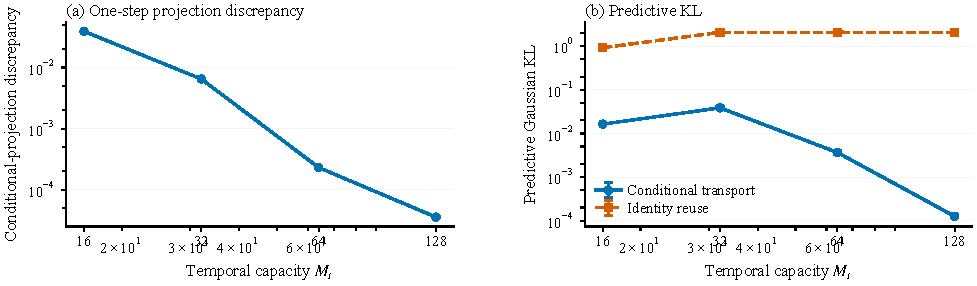
\includegraphics[width=0.98\textwidth]{figures/mechanism_diagnostics_two_panel.pdf}
\captionof{figure}{Transfer diagnostics. (a) One-step conditional-projection discrepancy. (b) Predictive Gaussian KL to the current-representation reference across temporal capacities for conditional transport and identity reuse. Conditional transport is non-monotone across the sweep, while identity reuse remains at order-one KL for $M_t\ge32$.}
\label{fig:transfer_solver_diagnostics}
\end{center}

\FloatBarrier
\clearpage

\subsection{Implementation efficiency audit}

The archived short-batch implementation audit at
$M_s=M_t=128$ on an RTX~4090 reports the ST-SVGP and KronHiPPO-STGP accuracy,
training wall time, profiler count, and peak reserved GPU memory from the same
audit record. This is an implementation-level comparison rather
than a framework-neutral complexity benchmark: the profiler column reports
supported-operation counts from the corresponding implementations and does not
represent complete hardware instruction-level FLOPs. The reported $40.4\times$
difference is therefore interpreted as a profiler-count ratio, while the
wall-clock and peak-memory ratios are measured implementation outcomes.

\begin{center}
\captionof{table}{Archived ERA5 short-batch implementation audit at $M_s=M_t=128$ on an RTX~4090. Accuracy and efficiency entries within each row come from the same audit record. \texttt{Train} denotes recorded training wall time, \texttt{Profiler GFLOPs/step} denotes supported-operation profiler counts, and \texttt{Peak} denotes reserved GPU memory.}
\label{tab:practical-efficiency}
\resizebox{0.82\textwidth}{!}{%
\begin{tabular}{@{}lrrrr@{}}
\toprule
Method & RMSE & Train (s) & \shortstack{Profiler\\GFLOPs/step} & Peak (GiB) \\
\midrule
ST-SVGP & 0.0837 & 4,586.83 & 1,106.04 & 14.75 \\
\method & 0.0882 & 41.39 & 27.36 & 1.68 \\
\midrule
\textit{Relative difference} & $+5.4\%$ RMSE & $110.8\times$ faster & $40.4\times$ lower & $8.8\times$ lower \\
\bottomrule
\end{tabular}
}
\end{center}

Appendix Table~\ref{app:efficiency-online} reports a separate strict-online accounting over Tasks~2--10, including
end-to-end execution, per-block posterior-update latency, prediction time, GPU
memory, and persistent-state size. These online records use a different
measurement scope from the short-batch audit and are therefore not combined with
Table~\ref{tab:practical-efficiency}
to form a cross-hardware or architecture-independent speed ratio.

\begin{center}
\captionof{table}{Online efficiency summary for ERA5 Tasks~2--10 using the formal
method names. End-to-end timing includes the online blocks, while the GPU and
persistent-state columns are implementation-specific. These values should not
be interpreted as hardware-normalised cross-method speed ratios.}
\label{app:efficiency-online}
\small
\setlength{\tabcolsep}{5.0pt}
\begin{tabular}{@{}lrrrrr@{}}
\toprule
Method & End-to-end (s) & Iter./block (s) & Predict (s) & GPU MiB & State MiB \\
\midrule
OSGPR & 78.00 & 0.1923 & 20.270 & 657 & 0.25 \\
StreamingSGPR & 29.81 & 0.0336 & 1.414 & 816 & 0.25 \\
Official OHSVGP & 254.32 & 1.2312 & 12.398 & 1966 & 0.08 \\
\method & 79.52 & 0.0214 & 3.562 & 1067 & 19.16 \\
Kron-STGP & 61.06 & 0.0204 & 3.500 & 1069 & 20.92 \\
\bottomrule
\end{tabular}
\end{center}
\FloatBarrier


\end{document}














